\documentclass[oneside]{book}

% PACKAGES
\usepackage[german,english]{babel}
\usepackage[utf8]{inputenc}
\usepackage{amsmath}
\usepackage{amsfonts}
\usepackage{amssymb}
\usepackage{amsthm}
\usepackage{marvosym}
\usepackage{tikz}
\usetikzlibrary{automata,arrows,positioning}
\usepackage{hyperref}
\usepackage{fancyhdr}
\usepackage[nottoc]{tocbibind}
\usepackage{environ}
\usepackage{algorithm}
\usepackage{algpseudocode}
\usepackage{pdfpages}
\usepackage{subcaption}
\usepackage[toc,page]{appendix}

\usepackage{geometry}

% COMMANDS
\newcommand{\enquote}[1]{``#1''}

% Quotient classes
\newcommand{\bigslant}[2]{{\raisebox{.2em}{$#1$}\left/\raisebox{-.2em}{$#2$}\right.}}
%\bigslant{A}{B}


% THEOREM STYLES
\newtheoremstyle{slplain}% name
  {.6\baselineskip\@plus.2\baselineskip\@minus.2\baselineskip}% Space above
  {0}% Space below
  {\slshape}% Body font
  {}%Indent amount (empty = no indent, \parindent = para indent)
  {\bfseries}%  Thm head font
  {.}%       Punctuation after thm head
  { }%      Space after thm head: " " = normal interword space;
        %       \newline = linebreak
  {}%       Thm head spec

\theoremstyle{slplain}
\newtheorem{theorem}{Theorem}[section]
\newtheorem{lem}[theorem]{Lemma}
\newtheorem{appendixlem}{Lemma}[chapter]
\newtheorem{prop}[theorem]{Proposition}
\newtheorem{cor}[theorem]{Corollary}

\theoremstyle{definition}
\newtheorem{defn}{Definition}[section]
\newtheorem{conj}{Conjecture}
\newtheorem{exmp}{Example}[chapter]

\theoremstyle{remark}
\newtheorem*{rem}{Remark}
\newtheorem*{note}{Note}
\newtheorem{case}{Case}

%FIX HYPERREF
\AtBeginDocument{\let\textlabel\label}

% REMOVE PROOFS
\NewEnviron{killcontents}{}
%\let\proof\killcontents
%\let\endproof\endkillcontents


% DISALLOW LINE BREAKS
\relpenalty=9999
\binoppenalty=9999


\begin{document}



\title{State Space Reduction For Parity Automata}
\author{Christof Löding \and Andreas Tollkötter}
\institute{RWTH Aachen, Lehrstuhl 7 f\"ur Informatik}
\date{\today}

\maketitle





\begin{abstract}
	Exact minimization of $\omega$-automata is a difficult problem and heuristic algorithms are a subject of current research. We establish a framework to generalize the known notion of quotient automata and uniformly describe such algorithms. We investigate several approaches to reduce the state space of deterministic parity automata. These are based on extracting information from structures within the automaton, such as strongly connected components, coloring of the states, and equivalence classes of given relations, to determine states that can safely be merged. The description of these procedures consists of a theoretical analysis as well as data collected from experiments. 
	\keywords{foo \and bar}
\end{abstract}


\section{Introduction}

Finite automata are a long established computation model that dates back to sources such as \cite{McCulloch1990} and \cite{RabinScott1959}. A known problem for finite automata is state space reduction, referring to the search of a language-equivalent automaton which uses fewer states than the original object. For deterministic finite automata (DFA), not just reduction but minimization was solved in \cite{Hopcroft1971}. Regarding nondeterministic finite automata (NFA), \cite{JianRavikumar1991} proved the PSPACE-completeness of the minimization problem, which is why reduction algorithms such as \cite{ChamparnaudCoulon2004} and \cite{BonchiPous2013} are a popular alternative.

In his prominent work \cite{Buchi1966}, B\"uchi introduced the model of B\"uchi automata (BA) as an extension of finite automata to read words of one-sided infinite length. As these $\omega$-automata tend to have higher levels of complexity in comparison to standard finite automata, the potential gain of state space reduction is even greater. Similar to NFAs, exact minimization for deterministic B\"uchi automata was shown to be NP-complete in \cite{Schewe2010} and spawned heuristic approaches such as \cite{Schewe2010}, \cite{MayrClemente2012}, or \cite{EtessamiWilkeSchuller2001}. 

As \cite{Thomas1991} displays, deterministic B\"uchi automata are a strictly weaker model than nondeterministic Büchi automata. It is therefore interesting to consider different models of $\omega$-automata in which determinism is possible while maintaining enough power to describe all $\omega$-regular languages. 
Parity automata (PA) are one such model, a combination of B\"uchi automata and Moore automata (\cite{Moore56}), that use a parity function, assigning a number (called priority or color) to each state. The convention used in this paper is that even priorities correspond to \enquote{good} states while odd priorities correspond to \enquote{bad} states. The smallest priority that is seen infinitely often during a run defines its acceptance; if it is even, the run will be accepting, and if it is odd, the run will be rejecting.
\cite{Mostowski1991}, \cite{Thomas1997} showed that deterministic parity automata are indeed sufficient to recognize all $\omega$-regular languages. As for DBAs, the exact minimization problem for DPAs is NP-complete (\cite{Schewe2010}).

\vspace{5pt}

In this paper, we investigate multiple techniques of heuristic state space reduction for DPAs. We present a general framework to uniformly describe these algorithms in a transparent manner. As opposed to a black box which provides as output a reduced automaton for each input, the framework aims towards giving more precise information about how the reduced DPA comes to be. This in theory makes it easier to find structures in the DPAs which are responsible for the reduction being applicable.
The base of the framework was the notion of quotient automata, which, for a given congruence relation on the states, merges all states of each equivalence class into one single representative. For example, building the quotient automaton of a DFA with the relation defined by the Myhill-Nerode theorem \cite{} will yield the minimal DFA for that language.

Our proposal for this framework are merger functions which generalize quotient automata. Merger functions map sets of states in the original DPA, called the merge set, to other sets of states, called the candidate set. The easiest interpretation, which we refer to as representative merge, allows us to merge all states from the merge set into any single representative that is chosen from the candidate set.

The most basic merge simply adapts the algorithm from \cite{Hopcroft1971}. Every parity automaton can be interpreted as a Moore automaton which can then be minimized using said algorithm. In this context, we call the equivalence relation which considers two states to be equivalent if they are merged by this algorithm the \emph{Moore equivalence}. 

A simple merger function that is introduced is the \emph{skip merger} which takes an equivalence relation that implies language equivalence on the states as a parameter and from that builds a merger function. The idea of using one given equivalence relation on the states and refining it is used several times in the paper. This merge decides on one particular strongly connected component (SCC) of the automaton and removes all states of an equivalence class that do not lie in this SCC, essentially \enquote{skipping} all other SCCs.

We adapt the works of \cite{FritzWilke06}, who considered alternating parity automata, to our case of deterministic parity automata and find that there are sufficient differences to warrant a separate analysis. The \emph{delayed simulation merger} considers two states to be equal, if on every run from those states on a shared word, if one run visits a priority at some position, the other run must visit a priority at most as high at some point in the future. It then holds that both runs will see the same smallest priority infinitely often and therefore either both accept or both reject. It suffices to choose one representative of each such equivalence class that has minimal priority and build the quotient automaton with those representatives.

%The \emph{iterated Moore} merge uses the idea that on $\omega$-automata, states which are only visited finitely often are irrelevant to the acceptance of a state. In particular, trivial SCCs, i.e. states with no path back to itself, can have their priority freely changed without affecting the language of the automaton. The idea of this merger therefore is to loosen the constraints on those states and then build the usual Moore equivalence.

We bring up merging via \emph{path refinement}, which uses an existing equivalence class of some congruence relation and refines it to a point where states can safely be merged. This refinement occurs so that two states from the class are equivalent if on each path from that state back to the class, both states visit the same minimal priority. 

Another merger function is the \emph{threshold Moore merger}, which again refines an existing relation. Two states are considered to be equivalent under the refinement if a relaxation of Moore equivalence, that considers all priorities greater than some $k$ to be equal, matches them. In this case we require the two states to have equal priority and choose $k$ to be that exact value.

A similar but slightly different approach is the \emph{LSF} merger function. It removes the need for two states to have equal priority and instead takes the value $k$ as a parameter. On the other side it adds a requirement similar to that of the skip merger, in that the candidates of the merge are those that all lie in one single SCC if we modify the automaton to only contain those states of priority at least $k$.
\vspace{5pt}

%The thesis is structured as follows: In the first chapter, we define basics notations and conventions and present some data of our empirical testing environment used to collect practical data of each approach.
%In the second chapter, we establish some theoretical ground work that will be used by the rest of the thesis.
%After that, we present the algorithms for state space reduction, split into one chapter for each such procedure. Each such chapter is made up of at least three sections. The first section describes the idea and definition of the algorithm and proofs well behaving properties. The second section covers how to actually compute the reduction and provides a short run time analysis. The third section shows practical data to analyze \enquote{real world} usefulness. Potential other sections contain variants or extensions of the original procedure as well as potential open questions. 
%At the very end, the appendix includes small examples to show how the individual merger functions are computed and work.








\chapter{Basics}
In the first chapter, we define basics notations and conventions and present some data of our empirical testing environment used to collect practical data of each approach.
In the second chapter, we establish some theoretical ground work that will be used by the rest of the thesis.
After that, we present several algorithms for state space reduction, split into one chapter for each such procedure. Each such chapter is made up of at least three sections. The first section describes the idea and definition of the algorithm and proofs well behaving properties. The second section covers how to actually compute the reduction and provides a short run time analysis. The third section shows practical data to analyze \enquote{real world} usefulness. Potential other sections contain variants or extensions of the original procedure as well as potential open questions.

\chapter{Basic Definitions}

The first chapter defines fundamentals of this thesis and notation used later on.

\section{General Mathematical Terms}
As our main focus is $\omega$-words, we will require a small extension of natural numbers into the transfinite realm.

\subsection{Sets and Functions}
\begin{defn}
	The \emph{natural numbers} $\mathbb{N} = \{0, 1, 2, \dots\}$ are the set of all non-negative integers. We define $0 := \emptyset$, $1 := \{0\}$, $2 := \{0, 1\}$, and so forth.
	
	The value $\omega$ denotes the \enquote{smallest} infinity, $\omega := \mathbb{N}$. For all natural numbers, we write $n < \omega$ and $\omega \not < \omega$. Also, we sometimes use the convention $n + \omega = \omega$.
	
	We denote the set $\mathbb{N} \cup \{\omega\}$ by $\mathbb{N}_\omega$.
\end{defn}

\begin{defn}
	Let $X$ and $Y$ be two sets. We use the usual definition of union ($\cup$), intersection ($\cap$), and set difference ($\setminus$). If some domain ($X \subseteq D$) is clear in the context, we write $X^\complement = D \setminus X$.
	
	We use the cartesian product $X \times Y = \{ (x, y) \mid x \in X, y \in Y \}$.
	
	We write $X^Y$ for the set of all functions with domain $Y$ and range $X$. If we have a function $f : D \rightarrow \{0, 1\}$, then we sometimes implicitly use it as a set $X \subseteq D$ with $x \in X$ iff $f(x) = 1$. In particular, $2^Y$ is the powerset of $Y$.
\end{defn}

\begin{defn}
	Let $f : D \rightarrow R$ be a function and let $X \subseteq D$ and $Y \subseteq R$. We describe by $f(X) = \{ f(x) \in R \mid x \in X\}$ and $f^{-1}(Y) = \{ x \in D \mid \exists y \in Y: f(x) = y \}$.
\end{defn}

\begin{defn}
	Let $X \subseteq D$ be a set. For $D' \subseteq D$, we define $X \upharpoonright_{D'} = X \cap D$. In particular, we use this notation for relations, e.g. $R \subseteq \mathbb{N} \times \mathbb{N}$ and $R \upharpoonright_{\{0\} \times \mathbb{N}}$.
	
	For a function $f : D \rightarrow R$, we write $f \upharpoonright_{D'}$ for the function $f' : D' \rightarrow R, x \mapsto f(x)$.
\end{defn}


\subsection{Relations and Orders}
\begin{defn}
	Let $X$ be a set. We call a set $R \subseteq X \times X$ a \emph{relation} over $X$. $R$ is
	\begin{itemize}
		\item \emph{reflexive}, if for all $x \in X$, $(x, x) \in R$.
		\item \emph{irreflexive}, if for all $x \in X$, $(x, x) \notin R$.
		\item \emph{symmetric}, if for all $(x, y) \in R$, also $(y, x) \in R$.
		\item \emph{asymmetric}, if for all $(x, y) \in R$, $(y, x) \notin R$.
		\item \emph{transitive}, if for all $(x, y), (y, z) \in R$, also $(x, z) \in R$.
		\item \emph{total}, if for all $x, y \in X$, $(x, y) \in R$ or $(y, x) \in R$ is true.
	\end{itemize}
	
	We call $R$ 
	\begin{itemize}
		\item a \emph{partial order}, if it is irreflexive, asymmetric, and transitive.
		\item a \emph{total order}, if it is a partial order and total.
		\item a \emph{preorder}, if it is reflexive and transitive.
		\item a \emph{total preorder}, if it is a preorder and total.
		\item an \emph{equivalence relation}, if it is a preorder and symmetric.
	\end{itemize}
	
	If $R$ is a partial order or a preorder, we call an element $x \in X$ \emph{minimal} (w.r.t. $R$), if for all $y \in X$, $(y, x) \in R$ implies $(x, y) \in R$. Similarly, we call it \emph{maximal}, if for all $y \in X$, $(x, y) \in R$ implies $(y, x) \in R$. 
	
	We call $x$ the \emph{minimum} of $R$ if for all $y \neq x$, $(y, x) \in R$. We write $x = \min_R X$.
\end{defn}

\begin{defn}
	Let $R$ be a partial order over $X$. We call a set $S \subseteq Y$ an \emph{extension of $R$ to $Y$} if $X \subseteq Y$, $R \subseteq S$, and $S$ is a partial order over $Y$. We use the same notation for total orders, preorders, and total preorders.
\end{defn}

\begin{defn}
	Let $R$ be an equivalence relation over $X$. $R$ implicitly forms a partition of $X$ into \emph{equivalence classes}. For an element $x \in X$, we call $[x]_R := \{ y \in X \mid (x, y) \in R \}$ the equivalence class of $x$. We denote the set of equivalence classes by $\mathfrak{C}(R) = \{ [x]_R \mid x \in R \}$.
\end{defn}





\section{Words and Languages}
\begin{defn}
	A non-empty set of symbols can be called an \emph{alphabet}, which we will denote by a variable $\Sigma$ most of the time. As symbols, we usually use lower case letters, i.e. $a$ or $b$.
	
	A \emph{finite word}, usually denoted by $u$, $v$, or $w$, over an alphabet $\Sigma$ is a function $w : n \rightarrow \Sigma$ for some $n$. We call $n$ the \emph{length} of $w$ and write $|w| = n$. The unique word of length $0$ is called \emph{empty word} and is written as $\varepsilon$.
	
	Given $\Sigma^n = \{ w \mid w \text{ is a word of length } n \text{ over } \Sigma \}$, we define $\Sigma^* = \bigcup\limits_{n \in \mathbb{N}} \Sigma^n$ as the set of all finite words over $\Sigma$. 
\end{defn}

\begin{defn}
	An \emph{$\omega$-word}, usually denoted by $\alpha$ or $\beta$, over an alphabet $\Sigma$ is a function $\alpha : \omega \rightarrow \Sigma$. $\omega$ is the length of $\alpha$ and we write $|\alpha| = \omega$. The set $\Sigma^\omega$ then describes the set of all $\omega$-words over $\Sigma$. 
\end{defn}

\begin{defn}
	A \emph{language} over an alphabet $\Sigma$ is a set of words $L \subseteq \Sigma^* \cup \Sigma^\omega$. In the context we use it should always be clear whether we are using finite words or $\omega$-words.
\end{defn}

\begin{defn}
	Let $v, w \in \Sigma^*$ and $w_i \in \Sigma^*$ for all $i \in \mathbb{N}$ be words over $\Sigma$ and $\alpha \in \Sigma^\omega$ be an $\omega$-word over $\Sigma$.
	
	The \emph{concatenation} of $v$ and $w$ (denoted by $v \cdot w$) is a word $u$ such that:
	\begin{align*}
	u : |v|+|w| \allowbreak \rightarrow \Sigma, i \mapsto 
	\begin{cases}
		v(i) & \text{if } i < |v| \\
		w(i-|v|) & \text{else}
	\end{cases}
	\end{align*}

	The \emph{concatenation} of $w$ and $\alpha$ (denoted by $w \cdot \alpha$) is an $\omega$-word $\beta$ such that:
	\begin{align*}
	\beta : \mathbb{N} \rightarrow \Sigma, i \mapsto 
	\begin{cases}
		w(i) & \text{if } i < |w| \\
		\alpha(i-|w|) & \text{else}
	\end{cases}
	\end{align*}
	
	For some $n \in \mathbb{N}$, the \emph{$n$-iteration} of $w$ (denoted by $w^n$) is a word $u$ such that:
	\begin{align*}
		u : |w|^n \rightarrow \Sigma, i \mapsto w(i \mod |w|)
	\end{align*}
	
	The \emph{$\omega$-iteration} of $w$ (denoted by $w^\omega$) is an $\omega$-word $\alpha$ such that:
	\begin{align*}
		\beta : \mathbb{N} \rightarrow \Sigma, i \mapsto w(i \mod |w|)
	\end{align*}
\end{defn}

\vspace{20pt}
For the purpose of easier notation and readability, we write singular symbols as words, i.e. for an $a \in \Sigma$ we write $a$ for the word $w_a : \{0\} \rightarrow \Sigma, i \mapsto a$.\\
We also abbreviate $v \cdot w$ to $vw$ and $w \cdot \alpha$ to $w \alpha$. Further, we use $\alpha \cdot \varepsilon = \alpha$ for $\alpha \in \Sigma^\omega$.
\vspace{10pt}

\begin{defn}
	Let $L, K \subseteq \Sigma^*$ be a language and $U \subseteq \Sigma^\omega$ be an $\omega$-language.\\
	The \emph{concatenation} of $L$ and $K$ is $L \cdot K = \{ u \in \Sigma^* \mid \text{There are } v \in L \text{ and } \allowbreak w \in K \text{ such that } u = v \cdot w\}$.\\
	The \emph{concatenation} of $L$ and $U$ is $L \cdot U = \{ \alpha \in \Sigma^\omega \mid \text{There are } w \in L \text{ and } \allowbreak \beta \in U \text{ such that } \alpha = w \cdot \beta\}$.\\
	For some $n \in \mathbb{N}$, the \emph{$n$-iteration} of $L$ is $L^n = \{ w \in \Sigma^* \mid \text{There is } v \in L \text{ such that } w = v^n\}$.\\
	The \emph{Kleene closure} of $L$ is $L^* = \bigcup\limits_{n \in \mathbb{N}} L^n$.\\
\end{defn}

\begin{defn}
	Let $w \in \Sigma^* \cup \Sigma^\omega$ be a word. We define a substring or subword of $w$ for some $n \leq m \leq |w|$ as $w[n, m] = w(n) \cdot w(n+1) \cdots w(m-1)$. In the case that $m = |w| = \omega$, it is simply $w[n, m] = w(n) \cdot w(n+1) \cdots$. Note that for $n = m$, we have $w[n, m] = \varepsilon$.
\end{defn}

\begin{defn}
	Let $v, w \in \Sigma^* \cup \Sigma^\omega$ be words. We call $v$ 
	\begin{itemize}
		\item a \emph{prefix} of $w$, if there is an $n \in \mathbb{N}_\omega$ with $v = w[0, n]$.
		\item a \emph{suffix} of $w$, if there is an $n \in \mathbb{N}_\omega$ with $v = w[n, |w|]$.
		\item an \emph{infix} of $w$, if there are $n, m \in \mathbb{N}_\omega$ with $v = w[n, m]$.
	\end{itemize}
\end{defn}

\begin{defn}
	The \emph{occurrence set} of a word $w \in \Sigma^* \cup \Sigma^\omega$ is the set of symbols which occur at least once in $w$. 
	$$\text{Occ}(w) = \{ a \in \Sigma \mid \text{There is an } n \in |w| \text{ such that } w(n) = a \text{.}\}$$
	
	The \emph{infinity set} of a word $w \in \Sigma^\omega$ is the set of symbols which occur infinitely often in $w$.
	$$\text{Inf}(w) = \{ a \in \Sigma \mid \text{For every } n \in \mathbb{N} \text{ there is a } m > n \text{ such that } w(m) = a \text{.}\}$$
\end{defn}


\section{Automata}

\begin{defn}
	Let $Q$ be a set, $\Sigma$ an alphabet, and $\delta : Q \times \Sigma \rightarrow Q$ a function. We call $\mathcal{S} = (Q, \Sigma, \delta)$ a \emph{deterministic transition structure}. We call $Q$ the states or state space.
	
	For $q \in Q$ and a word $w \in \Sigma^* \cup \Sigma^\omega$, we call $\rho \in Q^{1+|w|}$ the \emph{run} of $\mathcal{S}$ on $w$ starting in $q$ if $\rho(0) = q$ and for all $i$, $\rho(i+1) = \delta(\rho(i), w(i))$.
\end{defn}

\begin{defn}
	Let $\mathcal{S} = (Q, \Sigma, \delta)$ be a deterministic transition structure. For a set $\Omega \subseteq Q^* \cup Q^\omega$, we say that $\mathcal{S}$ has acceptance condition $\Omega$.
	
	We say that a run $\rho$ of $\mathcal{A}$ on some $w \in \Sigma^*$ is \emph{accepting}, if $\rho \in \Omega$; otherwise, the run is \emph{rejecting}. In either case, we say that $\mathcal{A}$ accepts or rejects $w$. 
	
	The \emph{language} of $\mathcal{A}$ with $\Omega$ from $q \in Q$ is the set of all words and $\omega$-words that are accepted by $\mathcal{A}$ from $q$.
\end{defn}

\begin{defn}
	Let $\mathcal{S} = (Q, \Sigma, \delta)$ be a deterministic transition structure. A \emph{strongly connected component}, or SCC, is a set $S \subseteq Q$ such that for all $p, q \in S$, there is a $w \in \Sigma^*$ with $\delta^*(p, w) = q$.
	
	An SCC $S$ is \emph{trivial} if it contains only one state $q$ and $\delta(q, a) \neq q$ for all $a \in \Sigma$.
\end{defn}

\begin{defn}
	A \emph{deterministic finite automaton} (or DFA) is a tuple $\mathcal{A} = (Q, \Sigma, \delta, F)$, where $F \subseteq Q$, such that $(Q, \Sigma, \delta)$ is a deterministic transition structure and has acceptance condition $\Omega = \{ \rho \in Q^* \mid \rho(|\rho|+1) \in F \}$. For the language of $(Q, \Sigma, \delta)$ with $\Omega$ from $q$, we write $L(\mathcal{A}, q)$.
\end{defn}

\begin{defn}
	A \emph{deterministic parity automaton} (or DPA) is a tuple $\mathcal{A} = (Q, \Sigma, \delta, c)$, where $c : Q \rightarrow \mathbb{N}$, such that $(Q, \Sigma, \delta)$ is a deterministic transition structure and has acceptance condition $\Omega = \{ \rho \in Q^* \mid \min \text{Inf}(c(\rho)) \text{ is even} \}$. For the language of $(Q, \Sigma, \delta)$ with $\Omega$ from $q$, we write $L(\mathcal{A}, q)$.
	
	We call the DPA a \emph{B\"uchi automaton} (or DBA) if $c(Q) \subseteq \{0, 1\}$. In that case, we use $F$ instead of $c$.
\end{defn}

\begin{defn}
	Let $\mathcal{S} = (Q, \Sigma, \delta)$ be a deterministic transition structure. We define $\delta^* : Q \times \Sigma^* \rightarrow Q$ as $\delta^*(q, \varepsilon) = q$ and $\delta^*(q, w \cdot a) = \delta(\delta^*(q, w), a)$.
\end{defn}

\begin{defn}
	Let $\mathcal{A} = (Q, \Sigma, \delta, c)$ be a DPA. We define $c^* : Q \times (\Sigma^* \cup \Sigma^\omega) \rightarrow (\mathbb{N}^* \cup \mathbb{N}^\omega)$ as $c^*(q, w) : 1+|w| \rightarrow \mathbb{N}, i \mapsto c(\delta^*(q, w[0, i]))$.
\end{defn}

\begin{defn}
	Let $\mathcal{S} = (Q, \Sigma, \delta)$ be a deterministic transition structure and $P \subseteq Q$. We define $\mathcal{S} \upharpoonright_P = (P, \Sigma, \delta')$ as a transition structure in which $\delta'$ might only be a partial function. We set $\delta'(p, a) = \delta(p, a)$ if $\delta(p, a) \in P$, or undefined otherwise.
\end{defn}


\vspace{1cm}




\section{Experimental Setup} %TODO
Even though the focus of this thesis lies in theoretical research, we consider it important to at least roughly analyze the practical \enquote{real world} efficiency of ever yalgorithm. All of them were implemented and tested on a set of deterministic parity automata.

The programming language of choice was C++14. The source code can be found in \cite{Tollkoetter2018}. The computer used to run the tests was an Arch Linux 4.19.4 64 bit machine powered by an AMD Ryzen 5 1600 processor and 16 GB DDR4-2400 RAM.


Several automata generated randomly using different parameters were used in the testing process. Three major different techniques of generation were used:

\begin{enumerate}
	\item Use Spot (\cite{duret.16.atva2}) to generate a random DPA. (called \textsf{gendet})
	\item Use Spot to generate a random non-deterministic B\"uchi automaton and use Spot again to convert it to a DPA. (called \textsf{detspot})
	\item Use Spot to generate a random non-deterministic B\"uchi automaton and use nbautils (\cite{Pirogov2018}) to convert it to a DPA. (called \textsf{detnbaut})
\end{enumerate}

Figures \ref{fig:rawstats:rawstats_size}, \ref{fig:rawstats:rawstats_prios}, \ref{fig:rawstats:rawstats_sccs}, \ref{fig:rawstats:rawstats_langclasnum} and \ref{fig:rawstats:rawstats_avg_langclassize} present some information about the automata. Regarding the number of states we stopped the generation at about 100 states, as most algorithms become too slow at that point. For the detnbaut set, the path refinement procedure can be sped up which is why the upper limit is higher. We elaborate this point in the relevant section.

The number of priorities is rather small in general. For gendet, we intentionally limited the number to 4 to mimic real world behavior that can be found in the detnbautils set. In comparison to nbautils, Spot does not perform priority reduction on the determinization result which explains why the detspot automata use more priorities in general.

The number of SCCs is consistently small among all three sets. detspot and gendet contain a few examples of automata with up to 60 SCCs but these are extreme outliers. This low number of SCCs is important to consider, as multiple of the algorithms such as the skip merger perform better the less connected the automaton is.

Finally, the average size of equivalence classes $\mathfrak{C}(\equiv_L)$. Again, this is of relevance to some of the reduction algorithms such as LSF as only states which are language equivalent can be merged. We can observe that the gendet set almost entirely consists of trivial classes (i.e. classes of size 1) while detspot and detnbaut show more promise in that regard.

\vspace{5pt}

Besides the three classes of data sets that we described above, we also looked at special families of automata that are specifically designed to be difficult to minimize; see \cite{Michel1988}. Unfortunately, these automata proved to be too difficult for our procedures and almost no algorithm could achieve any reduction on an automaton of any size. Thus, we will not discuss these results in any more detail in the upcoming chapters.

\begin{figure}
	\centering
	\begin{minipage}{0.49\textwidth}
		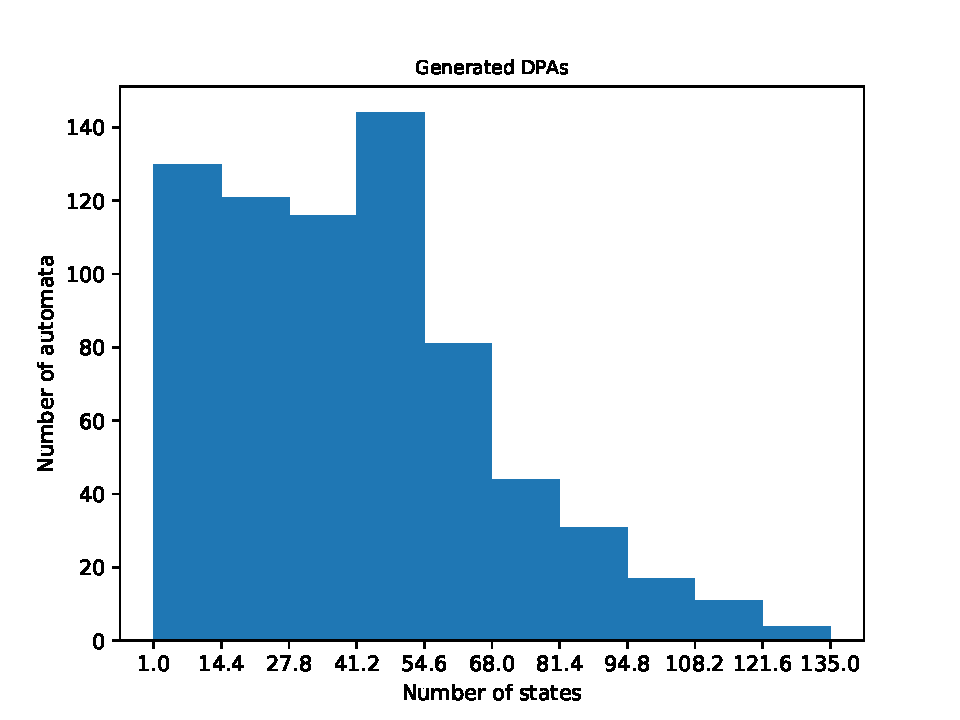
\includegraphics[page=1,height=.3\textheight]{../data/analysis/rawstats_gendet.pdf} 
		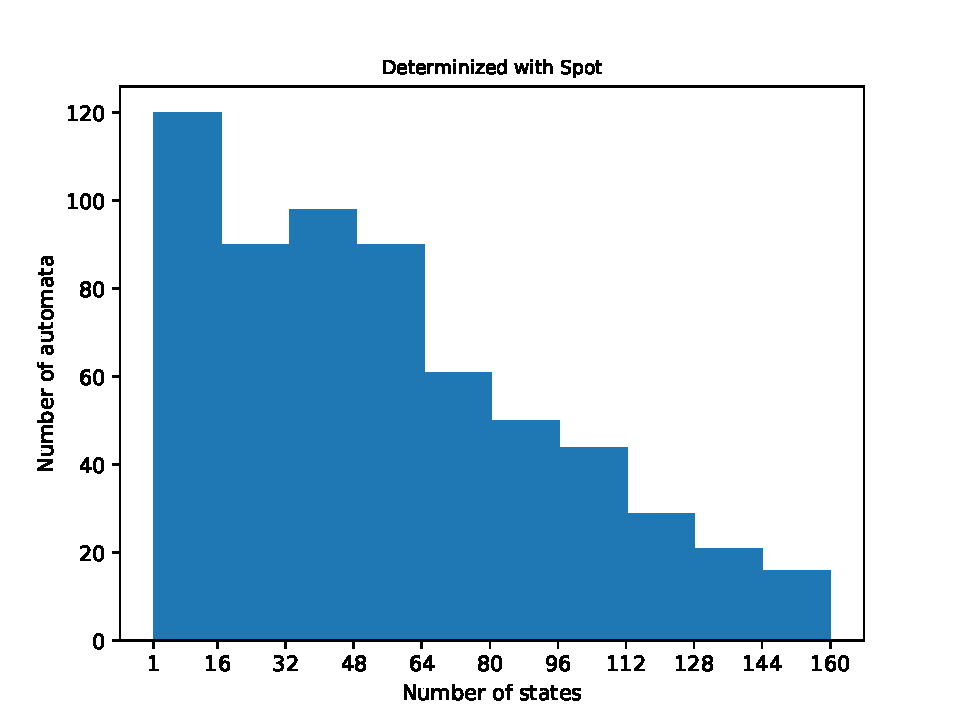
\includegraphics[page=1,height=.3\textheight]{../data/analysis/rawstats_detspot.pdf} 
		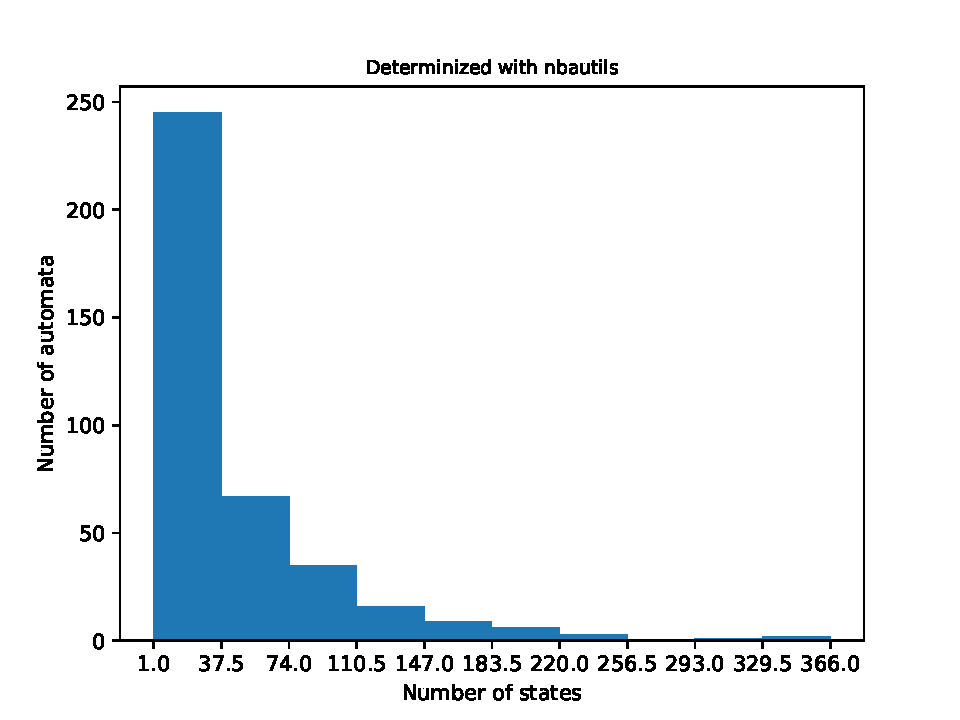
\includegraphics[page=1,height=.3\textheight]{../data/analysis/rawstats_detnbaut.pdf}
		\caption{Sizes of the automata in the testing environment.}
		\label{fig:rawstats:rawstats_size}
	\end{minipage}
	\hfill
	\begin{minipage}{0.49\textwidth}
		\includegraphics[page=2,height=.3\textheight]{../data/analysis/rawstats_gendet.pdf} 
		\includegraphics[page=2,height=.3\textheight]{../data/analysis/rawstats_detspot.pdf} 
		\includegraphics[page=2,height=.3\textheight]{../data/analysis/rawstats_detnbaut.pdf}
		\caption{Number of priorities in the automata in the testing environment.}
		\label{fig:rawstats:rawstats_prios}
	\end{minipage}
\end{figure}

\begin{figure}
	\centering
	\begin{minipage}{0.49\textwidth}
		\includegraphics[page=3,height=.3\textheight]{../data/analysis/rawstats_gendet.pdf} 
		\includegraphics[page=3,height=.3\textheight]{../data/analysis/rawstats_detspot.pdf} 
		\includegraphics[page=3,height=.3\textheight]{../data/analysis/rawstats_detnbaut.pdf}
		\caption{Number of SCCS in the automata in the testing environment.}
		\label{fig:rawstats:rawstats_sccs}
	\end{minipage}
	\hfill
	\begin{minipage}{0.49\textwidth}
		\includegraphics[page=4,height=.3\textheight]{../data/analysis/rawstats_gendet.pdf} 
		\includegraphics[page=4,height=.3\textheight]{../data/analysis/rawstats_detspot.pdf} 
		\includegraphics[page=4,height=.3\textheight]{../data/analysis/rawstats_detnbaut.pdf}
		\caption{Number of classes in $\mathfrak{C}(\equiv_L)$ that contain more than one state.}
		\label{fig:rawstats:rawstats_langclasnum}
	\end{minipage}
\end{figure}


\begin{figure}
	\centering
	\begin{minipage}{0.49\textwidth}
		\includegraphics[page=5,height=.3\textheight]{../data/analysis/rawstats_gendet.pdf} 
		\includegraphics[page=5,height=.3\textheight]{../data/analysis/rawstats_detspot.pdf} 
		\includegraphics[page=5,height=.3\textheight]{../data/analysis/rawstats_detnbaut.pdf}
		\caption{Average size of $\equiv_L$-classes of the automata in the testing environment.}
		\label{fig:rawstats:rawstats_avg_langclassize}
	\end{minipage}
\end{figure}


 



\chapter{General Theory}
\section{Equivalence Relations}

In general, we use the symbol $\equiv$ to denote equivalence relations, mostly between states of an automata. In general, we have automata $\mathcal{A}$ and $\mathcal{B}$ with states $p$ and $q$ from there respective state spaces. Our relations are then defined on $(\mathcal{A}, p) \equiv (\mathcal{B}, q)$.

\begin{defn}
	Assuming that $\mathcal{A}$ is a fixed automaton that is obvious in context and $p$ and $q$ are both states in $\mathcal{A}$, we shorten $(\mathcal{A}, p) \equiv (\mathcal{A}, q)$ to $p \equiv q$.
	
	Furthermore, we write $\mathcal{A} \equiv \mathcal{B}$ if for every $p$ in $\mathcal{A}$ there is a $q$ in $\mathcal{B}$ such that $(\mathcal{A}, p) \equiv (\mathcal{B}, q)$; and the same holds with $\mathcal{A}$ and $\mathcal{B}$ exchanged.
\end{defn}

\begin{defn}
	Let $\mathcal{A} = (Q_1, \Sigma, \delta_1)$ and $\mathcal{B} = (Q_2, \Sigma, \delta_2)$ be deterministic transition structures and let $\sim$ be an equivalence relation. We call $\sim$ a \emph{congruence relation} if for all $(\mathcal{A}, p) \sim (\mathcal{B}, q)$ and all $a \in \Sigma$, also $(\mathcal{A}, \delta_1(p, a)) \sim (\mathcal{B}, \delta_2(q, a))$.
\end{defn}

\begin{defn}
	Let $\sim$ be an equivalence relation. We define the \emph{congruence refinement} of $\sim$ as $\approx$ with $(\mathcal{A}, p) \approx (\mathcal{B}, q)$ iff for all $w \in \Sigma^*$, $(\mathcal{A}, \delta_1^*(p, w)) \sim (\mathcal{B}, \delta_2(q, w))$.
\end{defn}

\begin{lem}
	For a given equivalence relation $\sim$, the congruence refinement of $\sim$ is a congruence relation.
\end{lem}

\begin{proof}
	Assume towards a contradiction that there are $(\mathcal{A}, p) \approx (\mathcal{B}, q)$ such that $(\mathcal{A}, \delta_1(p, a)) \not\approx (\mathcal{B}, \delta_2(q, a))$. Thus, there is a $w \in \Sigma^*$ with $(\mathcal{A}, \delta_1^*(\delta_1(p, a), w)) \not\sim (\mathcal{B}, \delta_2(\delta_2(q, a), w))$. This means $(\mathcal{A}, \delta_1^*(p, aw)) \not\sim (\mathcal{B}, \delta_2(q, aw))$ and therefore $(\mathcal{A}, p) \not\approx (\mathcal{B}, q)$.
\end{proof}

\begin{lem}
	For a given equivalence relation $\sim$, the congruence refinement on a single automaton $\mathcal{A}$ can be computed in $\mathcal{O}(|\mathcal{A}| \cdot \log |\mathcal{A}|)$.
	\label{lem:general:congref_in_nlogn}
\end{lem}

\begin{proof}
	We refer to \cite{Hopcroft1971}, which describes a special case where $p \sim q$ iff $c(p) = c(q)$.
\end{proof}


\vspace{15pt}
The following is a comprehensive list of all relevant equivalence relations that we use.

\begin{itemize}
	\item Language equivalence, $\equiv_L$. Defined below.
	\item Moore equivalence, $\equiv_M$. Defined below.
	\item Priority almost equivalence, $\equiv_\text{\Ankh}$. Defined below.
	\item Delayed simulation equivalence, $\equiv_\text{de}$. Defined in chapter \ref{chap:fritzwilke}.
	\item Delayed simulation equivalence with resets, $\equiv_\text{deR}$. Defined in chapter \ref{chap:fritzwilke}.
	\item Iterated Moore equivalence, $\equiv_\text{IM}$. Defined in chapter \ref{chap:imoore}.
	\item Path refinement equivalence, $\equiv_\text{PR}$. Defined in chapter \ref{chap:pr}.
	\item Threshold Moore equivalence, $\equiv_\text{TM}^\sim$. Defined in chapter \ref{chap:tm}.
	\item Labeled SCC filter equivalence, $\equiv_\text{LSF}^{k,\sim}$. Defined in chapter \ref{chap:lsf}.
\end{itemize}

Immediately we define the three first of these relations and show that they are computable.

\vspace{5pt}

\subsection{Language Equivalence}

\begin{defn}
	Let $\mathcal{A}$ and $\mathcal{B}$ be $\omega$-automata. We define \emph{language equivalence} as $(\mathcal{A}, p) \equiv_L (\mathcal{B}, q)$ if and only if for all words $\alpha \in \Sigma^\omega$, $\mathcal{A}$ accepts $\alpha$ from $p$ iff $\mathcal{B}$ accepts $\alpha$ from $q$.
\end{defn}

\begin{lem}
	$\equiv_L$ is a congruence relation.
	\label{lem:general:L_congruence}
\end{lem}

\begin{proof}
	It is obvious that $\equiv_L$ is an equivalence relation. For two states $(\mathcal{A}, p) \equiv_L (\mathcal{B}, q)$ and some successors $p' = \delta_1(p, a)$ and $q' = \delta_2(q, a)$, it must be true that $(\mathcal{A}, p') \equiv_L (\mathcal{B}, q')$. Otherwise there is a word $\alpha \in \Sigma^\omega$ that is accepted from $p'$ and rejected from $q'$ (or vice-versa). Then $a \cdot \alpha$ is rejected from $p$ and accepted from $q$ and thus $p \not\equiv_L q$.
\end{proof}

\begin{lem}
	Language equivalence of a given DPA can be computed in $\mathcal{O}(|Q|^2 \cdot |c(Q)|^2)$.
\end{lem}

\begin{proof}
	The algorithm is based partially on \cite{HenzingerTelle1996}.
	
	Let $\mathcal{A} = (Q, \Sigma, \delta, c)$ be the DPA that we want to compute $\equiv_L$ on. We construct a labeled deterministic transition structure $\mathcal{B} = (Q \times Q, \Sigma, \delta', d)$ with $\delta'((p_1, p_2), a) = (\delta(p_1, a), \delta(p_2, a))$ and $d((p_1, p_2)) = (c(p_1), c(p_2)) \in \mathbb{N}^2$. Then, for every $i, j \in c(Q)$, let $\mathcal{B}_{i,j} = \mathcal{B} \upharpoonright_{Q_{i,j}}$ with $Q_{i,j} = \{ (p_1, p_2) \in Q \times Q \mid c(p_1) \geq i, c(p_2) \geq j \}$, i.e. remove all states which have first priority less than $i$ or second priority less than $j$.
	
	For each $i$ and $j$, let $S_{i,j} \subseteq 2^{Q \times Q}$ be the set of all SCCs in $\mathcal{B}_{i,j}$ and let $S = \bigcup_{i,j} S_{i,j}$. From this set $S$, remove all SCCs $s \subseteq Q \times Q$ in which the parity of the smallest priority in the first component differs from the parity of the smallest priority in the second component. The \enquote{filtered} set we call $S'$. For any two states $p, q \in Q$, $p \not\equiv_L q$ iff there is a pair $(p', q') \in \bigcup S'$ that is reachable from $(p, q)$ in $\mathcal{B}$.
	
	We omit the correctness proof of the algorithm here. Regarding the runtime, observe that $\mathcal{B}$ has size $\mathcal{O}(|Q|^2)$ and we create $\mathcal{O}(|c(Q)|^2)$ copies of it. All other steps like computing the SCCs can then be done in linear time in the size of the automata, which brings the total to $\mathcal{O}(|Q|^2 \cdot |c(Q)|^2)$.
\end{proof}

\vspace{5pt}

\subsection{Priority Almost Equivalence}

\begin{defn}
	Let $\mathcal{A} = (Q_1, \Sigma, \delta_1, c_1)$ and $\mathcal{B} = (Q_2, \Sigma, \delta_2, c_2)$ be DPAs. We define \emph{priority almost equivalence} as $(\mathcal{A}, p) \equiv_\text{\Ankh} (\mathcal{B}, q)$ if and only if for all words $\alpha \in \Sigma^\omega$, $c_1^*(p, \alpha)$ and $c_2^*(q, \alpha)$ differ at only finitely many positions.
\end{defn}

\begin{lem}
	Priority almost equivalence is a congruence relation.
	\label{lem:general:Ankh_congruence}
\end{lem}

\begin{proof} 
	It is obvious that $\equiv_\text{\Ankh}$ is an equivalence relation. For two states $(\mathcal{A}, p) \equiv_\text{\Ankh} (\mathcal{B}, q)$ and some successors $p' = \delta(p, a)$ and $q' = \delta(q, a)$, it must be true that $(\mathcal{A}, p') \equiv_\text{\Ankh} (\mathcal{B}, q')$. Otherwise there is a word $\alpha \in \Sigma^\omega$ such that $c_1^*(p', \alpha)$ and $c_2^*(q', \alpha)$ differ at infinitely many positions. Then $c_1^*(p, a \alpha)$ and $c_2^*(q, a \alpha)$ also differ at infinitely many positions and thus $(\mathcal{A}, p) \not\equiv_\text{\Ankh} (\mathcal{B}, q)$.
\end{proof}

The following definition is used as an intermediate step on the way to computing $\equiv_\text{\Ankh}$.

\begin{defn}
	Let $\mathcal{A} = (Q_1, \Sigma, \delta_1, c_1)$ and $\mathcal{B} = (Q_2, \Sigma, \delta_2, c_2)$ be DPAs. We define the deterministic Büchi automaton $\mathcal{A} \intercal \mathcal{B} = (Q_1 \times Q_2, \Sigma, \delta_\intercal, F_\intercal)$ with $\delta_\intercal((q_1, q_2), a) = (\delta_1(q_1, a), \delta_2(q_2, a))$. The transition structure is a common product automaton.
	
	The final states are $F_\intercal = \{ (p, q) \in Q_1 \times Q_2 \mid c_1(p) \neq c_2(q) \}$, i.e. every pair of states at which the priorities differ. 
\end{defn}

\begin{lem}
	$\mathcal{A} \intercal \mathcal{B}$ can be computed in time $\mathcal{O}(|Q_1| \cdot |Q_2|)$.
	\label{lem:general:intercal_runtime}
\end{lem}

\begin{proof}
	The definition already provides a rather straightforward description of how to compute $\mathcal{A} \intercal \mathcal{B}$. Each state only requires constant time (assuming that $\delta$ and $c$ can be evaluated in such) and has $|\mathcal{A}| \cdot |\mathcal{B}|$ many states.
\end{proof}

\begin{lem}
	Let $\mathcal{A} = (Q_1, \Sigma, \delta_1, c_1)$ and $\mathcal{B} = (Q_2, \Sigma, \delta_2, c_2)$ be DPAs. $(\mathcal{A}, p) \equiv_\text{\Ankh} (\mathcal{B}, q)$ iff $L(\mathcal{A} \intercal \mathcal{B}, (p, q)) = \emptyset$. 
	\label{lem:general:intercal_prioalmostequiv}
\end{lem}

\begin{proof}
	For the first direction of implication, let $L(\mathcal{A} \intercal \mathcal{B}, (p_0, q_0)) \neq \emptyset$, so there is a word $\alpha$ accepted by that automaton. Let $(p, q) (p_1, q_1) (p_2, q_2) \cdots$ be the accepting run on $\alpha$. Then $p p_1 \cdots$ and $q q_1 \cdots$ are the runs of $\mathcal{A}$ and $\mathcal{B}$ on $\alpha$ respectively. Whenever $(p_i, q_i) \in F_\intercal$, $p_i$ and $q_i$ have different priorities. As the run of the product automaton vists infinitely many accepting states, $\alpha$ is a witness for $p$ and $q$ being not priority almost-equivalent.
	
	For the second direction, let $p$ and $q$ be not priority almost-equivalent, so there is a witness $\alpha$ at which infinitely many positions differ in priority. Analogously to the first direction, this means that the run of $\mathcal{A} \intercal \mathcal{B}$ on the same word is accepting and therefore the language is not empty.
\end{proof}

\begin{cor}
	Priority almost equivalence of a given DPA can be computed in quadratic time.
\end{cor}

\begin{proof}
	By Lemma \ref{lem:general:intercal_runtime}, we can compute $\mathcal{A} \intercal \mathcal{A}$ in quadratic time. The emptiness problem for deterministic B\"uchi automata is solvable in linear time by checking reachability of loops that contain a state in $F$. 
\end{proof}

\vspace{5pt}

\subsection{Moore Equivalence}

\begin{defn}
	Let $\mathcal{A} = (Q_1, \Sigma, \delta_1, c_1)$ and $\mathcal{B} = (Q_2, \Sigma, \delta_2, c_2)$ be DPAs. We define \emph{Moore equivalence} as $(\mathcal{A}, p) \equiv_M (\mathcal{B}, q)$ if and only if for all words $w \in \Sigma^*$, $c_1(\delta^*(p, w)) = c_2(\delta^*(q, w))$.
\end{defn}

\begin{lem}
	Moore equivalence is the congruence refinement of $\sim$ with $(\mathcal{A}, p) \sim (\mathcal{B}, q)$ iff $c(p) = c(q)$.
\end{lem}

\begin{cor}
	$\equiv_M$ is a congruence relation.
	\label{cor:general:M_congruence}
\end{cor}

\begin{cor}
	Moore equivalence of a given DPA can be computed in log-linear time.
	\label{cor:general:M_loglin}
\end{cor}


\vspace{10pt}

\begin{theorem}
	$\equiv_M \,\subseteq\, \equiv_\text{\Ankh} \,\subseteq\, \equiv_L$
	\label{thm:general:M_subs_Ankh_subs_L}
\end{theorem}

\begin{proof}
	Let $\mathcal{A} = (Q_1, \Sigma, \delta_1, c_1)$ and $\mathcal{B} = (Q_2, \Sigma, \delta_2, c_2)$ be DPAs with states $q_1 \in Q_1$ and $q_2 \in Q_2$. 
	
	At first, let $(\mathcal{A}, q_1) \equiv_M (\mathcal{B}, q_2)$ and assume towards a contradiction that $(\mathcal{A}, q_1) \not\equiv_\text{\Ankh} (\mathcal{B}, q_2)$, so there is a word $\alpha \in \Sigma^\omega$ such that $c_1^*(q_1, \alpha)$ and $c_2^*(q_2, \alpha)$ differ at infinitely many positions. In particular, there is some $w \sqsubseteq \alpha$ such that $c_1(\delta_1^*(q_1, w)) \neq c_2(\delta_2^*(q_2, w))$. This would be a contradiction to $(\mathcal{A}, q_1) \equiv_M (\mathcal{B}, q_2)$.
	
	Now assume that $(\mathcal{A}, q_1) \equiv_\text{\Ankh} (\mathcal{B}, q_2)$ and let $\alpha \in \Sigma^\omega$. Let $\rho_1$ and $\rho_2$ be the runs of $\mathcal{A}$ and $\mathcal{B}$ on $\alpha$ starting in $q_1$ and $q_2$. Because $(\mathcal{A}, q_1) \equiv_\text{\Ankh} (\mathcal{B}, q_2)$ is true, there is a position $n$ such that $c_1(\rho_1[n,\omega]) = c_2(\rho_2[n,\omega])$ and therefore $\text{Inf}(c_1(\rho_1[n,\omega])) = \text{Inf}(c_2(\rho_2[n,\omega]))$, which means that the runs have the same acceptance. Thus, $(\mathcal{A}, q_1) \equiv_L (\mathcal{B}, q_2)$.
\end{proof}






\section{Representative Merge}

\begin{defn}
	Let $\mathcal{A} = (Q, \Sigma, \delta, c)$ be a DPA and let $\emptyset \neq C \subseteq M \subseteq Q$. Let $\mathcal{A}' = (Q', \Sigma, \delta', c')$ be another DPA. We call $\mathcal{A}'$ a \emph{representative merge of $\mathcal{A}$ w.r.t. $M$ by candidates $C$} if it satisfies the following:
	\begin{itemize}
		\item There is a state $r_M \in C$ such that $Q' = (Q \setminus M) \cup \{r_M\}$.
		\item $c' = c\upharpoonright_{Q'}$.
		\item Let $p \in Q'$ and $\delta(p, a) = q$. If $q \in M $, then $\delta'(p, a) = r_M$. Otherwise, $\delta'(p, a) = q$. 
	\end{itemize}
	
	We call $r_M$ the \emph{representative} of $M$ in the merge. We might omit $C$ and implicitly assume $C = M$.
\end{defn}

\begin{defn}
	Let $\mathcal{A} = (Q, \Sigma, \delta, c)$ be a DPA and let $\mu : D \rightarrow (2^\mathcal{Q} \setminus \emptyset)$ be a function for some $D \subseteq 2^Q$. We call $\mu$ a \emph{merger function} if 
	\begin{itemize}
		\item all sets in $D$ are pairwise disjoint; and
		\item for $U = \bigcup D$ and all sets $X \in D$, $\mu(X) \cap (U \setminus X) = \emptyset$
	\end{itemize}
	
	A DPA $\mathcal{A}'$ is a representative merge of $\mathcal{A}$ w.r.t. $\mu$ if there is an enumeration $X_1, \dots, X_{|D|}$ of $D$ and a sequence of automata $\mathcal{A}_0, \dots, \mathcal{A}_{|D|}$ such that $\mathcal{A}_0 = \mathcal{A}$, $\mathcal{A}_{|D|} = \mathcal{A}'$ and every $\mathcal{A}_{i+1}$ is a representative merge of $\mathcal{A}_i$ w.r.t. $X_{i+1}$ by candidates $\mu(X_{i+1})$.
\end{defn}

\vspace{5pt}

The following Lemma formally proofs that this definition actually makes sense, as building representative merges is commutative if the merge sets are disjoint.

\begin{lem}
	Let $\mathcal{A} = (Q, \Sigma, \delta, c)$ be a DPA and let $M_1, M_2 \subseteq Q$. Let $\mathcal{A}_1$ be a representative merge of $\mathcal{A}$ w.r.t. $M_1$ by some candidates $C_1$. Let $\mathcal{A}_{12}$ be a representative merge of $\mathcal{A}_1$ w.r.t. $M_2$ by some candidates $C_2$. If $M_1$ and $M_2$ are disjoint, then there is a representative merge $\mathcal{A}_2$ of $\mathcal{A}$ w.r.t. $M_2$ by candidates $C_2$ such that $\mathcal{A}_{12}$ is a representative merge of $\mathcal{A}_2$ w.r.t $M_1$ by candidates $C_1$.
\end{lem}

\begin{proof}
	By choosing the same representative $r_{M_1}$ and $r_{M_2}$ in the merges, this is a simple application of the definition.
\end{proof}

\begin{lem}
	Given a DPA $\mathcal{A}$ and a merger function $\mu : D \rightarrow 2^Q$ in suitable data structures, a representative merge of $\mathcal{A}$ w.r.t. $\mu$ can be computed in linear time.
	\label{lem:general:repmerge_lintime}
\end{lem}

\begin{proof}
	If for each $q \in Q$, we can find the $M \in D$ with $q \in M$ in constant time, and are also able to evaluate $\mu(M)$ in constant time (e.g. with a hash map), then building the representative merge comes down to iterating over all states in the automaton and checking their status in the sets in $D$ or their candidates. This can be done in linear time.
\end{proof}

\vspace{10pt}

The following Lemma, while simple to prove, is interesting and will find use in multiple proofs of correctness later on.

\begin{lem}
	Let $\mathcal{A}$ be a DPA. Let $\sim$ be a congruence relation on $Q$ and let $M \subseteq Q$ such that for all $x, y \in M$, $x \sim y$. Let $\mathcal{A}'$ be a representative merge of $\mathcal{A}$ w.r.t. $M$ by candidates $C$. Let $\rho$ and $\rho'$ be runs of $\mathcal{A}$ and $\mathcal{A}'$ on some $\alpha$. Then for all $i$, $(\mathcal{A}, \rho(i)) \sim (\mathcal{A}, \rho'(i))$.
	\label{lem:general:cong_stays_in_merge}
\end{lem}

\begin{proof}
	We use a proof by induction. For $i = 0$, we have $\rho(0) = q_0$ for some $q_0 \in Q$ and $\rho'(0) = r_{[q_0]_M}$. By choice of the representative, $q_0 \in M$ and $r_{[q_0]_M} \in M$ and thus $q_0 \sim r_{[q_0]_M}$.
	
	Now consider some $i+1 > 0$. Then $\rho'(i+1) = r_{[q]_M}$ for $q = \delta(\rho'(i), \alpha(i))$. By induction we know that $\rho(i) \sim \rho'(i)$ and thus $\delta(\rho(i), \alpha(i)) = \rho(i+1) \sim q$. Further, we know $q \sim r_{[q]_M}$ by the same argument as before. Together this lets us conclude in $\rho(i+1) \sim q \sim \rho'(i+1)$.
\end{proof}

\vspace{10pt}

The following is a comprehensive list of all relevant merger functions that we use.

\begin{itemize}
	\item Quotient merger, $\mu_\div^\sim$. Defined below.
	\item Moore merger, $\mu_M$. Defined below.
	\item Skip merger, $\mu_\text{skip}^\sim$. Defined in chapter \ref{chap:skipper}.
	\item Delayed simulation merger, $\mu_\text{de}$. Defined in chapter \ref{chap:fritzwilke}.
	\item Path refinement merger, $\mu_\text{PR}^\lambda$. Defined in chapter \ref{chap:pr}.
	\item Treshold Moore merger, $\mu_\text{TM}^\sim$. Defined in chapter \ref{chap:tm}.
	\item Labeled SCC Filter merger, $\mu_\text{LSF}^{k,\sim}$. Defined in chapter \ref{chap:lsf}.
\end{itemize}

\vspace{5pt}

\subsection{Quotient merger}
\begin{defn}
	Let $\sim$ be a congruence relation. We define the \emph{quotient merger} $\mu^\sim_\div : \mathfrak{C}(\sim) \rightarrow 2^Q, \kappa \mapsto \kappa$. 
\end{defn}


\begin{lem}
\label{lem:general:congrel_prio_implies_moore}
	Let $\mathcal{A} = (Q, \Sigma, \delta, c)$ be a DPA and let $\sim$ be a congruence relation such that $p \sim q$ implies $c(p) = c(q)$. Then $\mathcal{A}$ is Moore equivalent to every representative merge w.r.t. $\mu_\div^\sim$.
\end{lem} 

\begin{proof} 
	Let $\mathcal{A}' = (Q', \Sigma, \delta', c')$ be a representative merge. For every $q \in Q$, we prove that $(\mathcal{A}, q) \equiv_M (\mathcal{A}', r_{[q]_\sim})$. Since all states in $\mathcal{A}'$ are representatives of that form and every representative exists in $\mathcal{A}$ as well, this suffices to prove Moore equivalence.
	
	Let $\alpha \in \Sigma^\omega$ be a word and let $\rho$ and $\rho'$ be the runs of $\mathcal{A}$ and $\mathcal{A}'$ on $\alpha$ starting in $q$ and $r_{[q]_\sim}$. For every $i \in \mathbb{N}$, we have $\rho'(i) = [\rho(i)]_\sim$ and thus $c'(\rho'(i)) = c(\rho(i))$. Therefore, $\rho$ is accepting iff $\rho'$ is accepting.
\end{proof}



\subsection{Moore merger}
\begin{defn}
	We define the special \emph{Moore merger} $\mu_M = \mu_\div^{\equiv_M}$.
\end{defn}

\begin{lem}
	Let $\mathcal{A}$ be a DPA and let $\mathcal{A}'$ be a representative merge of $\mathcal{A}$ w.r.t. $\mu_M$. Then $\mathcal{A} \equiv_L \mathcal{A}'$.
\end{lem}

\begin{proof}
	Directly implied by Lemma \ref{lem:general:congrel_prio_implies_moore} and Theorem \ref{thm:general:M_subs_Ankh_subs_L}.
\end{proof}

\vspace{5pt}

In figure \ref{fig:general:empirical_moore_size_hist}, the efficiency of $\mu_M$ on different types of automata is shown. On the \textsf{gendet} and \textsf{detnbaut} classes, barely any state reduction is achieved. \textsf{gendet} lacks patterns in its automata and \textsf{detnbaut} already has certain minimization techniques applied during generation. \textsf{detspot} on the other hand shows some small but noticeable reduction. In figure \ref{fig:general:empirical_moore_reduct_abs}, we can see that the number of removed states is roughly proportional to the number of total states, which is no big surprise.

As is to be expected from Corollary \ref{cor:general:M_loglin} and confirmed in figure \ref{fig:general:empirical_moore_time}, the Moore merger is very easy to compute.


\begin{figure}
	\centering
	\begin{minipage}{0.49\textwidth}
		\includegraphics[page=6,height=.3\textheight]{../data/analysis/hopcroft/gendet_ap1.pdf} 
		\includegraphics[page=6,height=.3\textheight]{../data/analysis/hopcroft/detspot_ap1.pdf} 
		\includegraphics[page=6,height=.3\textheight]{../data/analysis/hopcroft/detnbaut_ap1.pdf} 
		\caption{State reduction of different automata using $\mu_M$.}
		\label{fig:general:empirical_moore_size_hist}
	\end{minipage}
	\hfill
	\begin{minipage}{0.49\textwidth}
		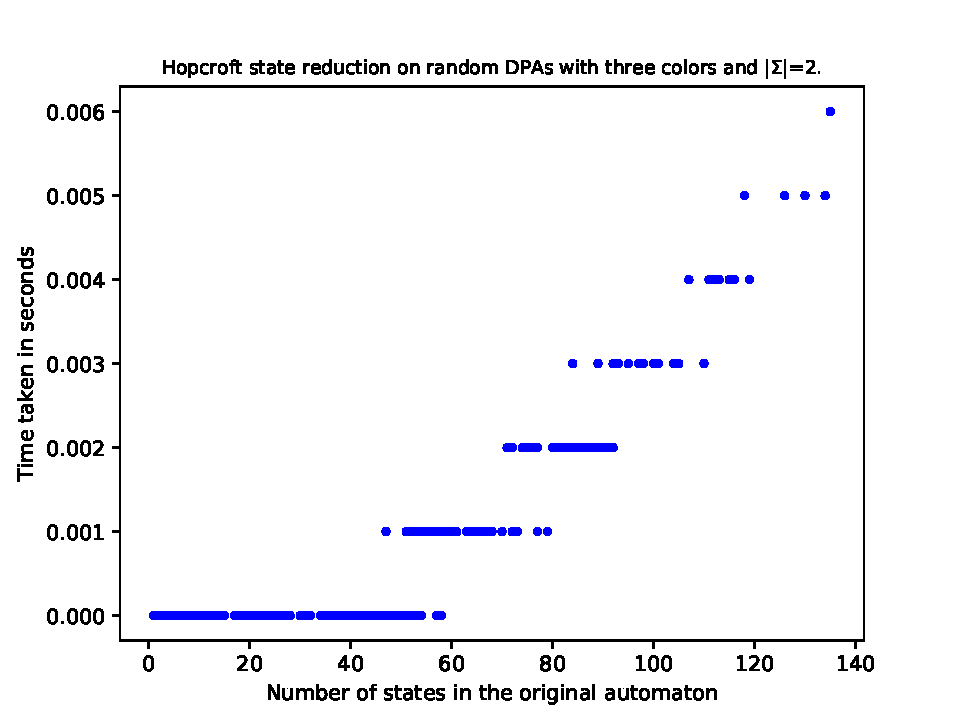
\includegraphics[page=1,height=.3\textheight]{../data/analysis/hopcroft/gendet_ap1.pdf} 
		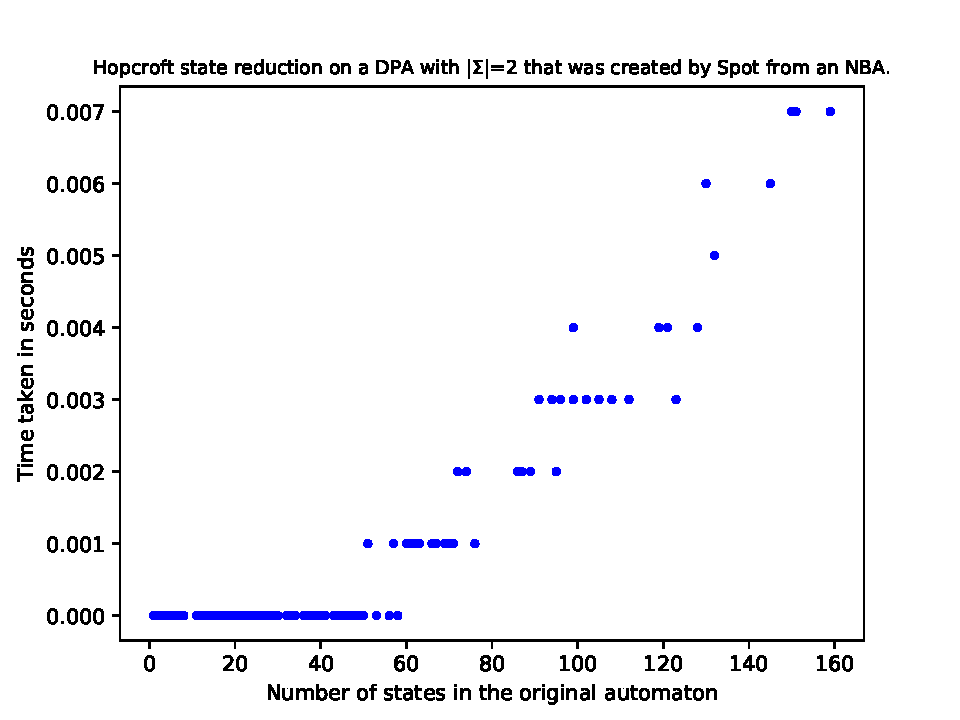
\includegraphics[page=1,height=.3\textheight]{../data/analysis/hopcroft/detspot_ap1.pdf} 
		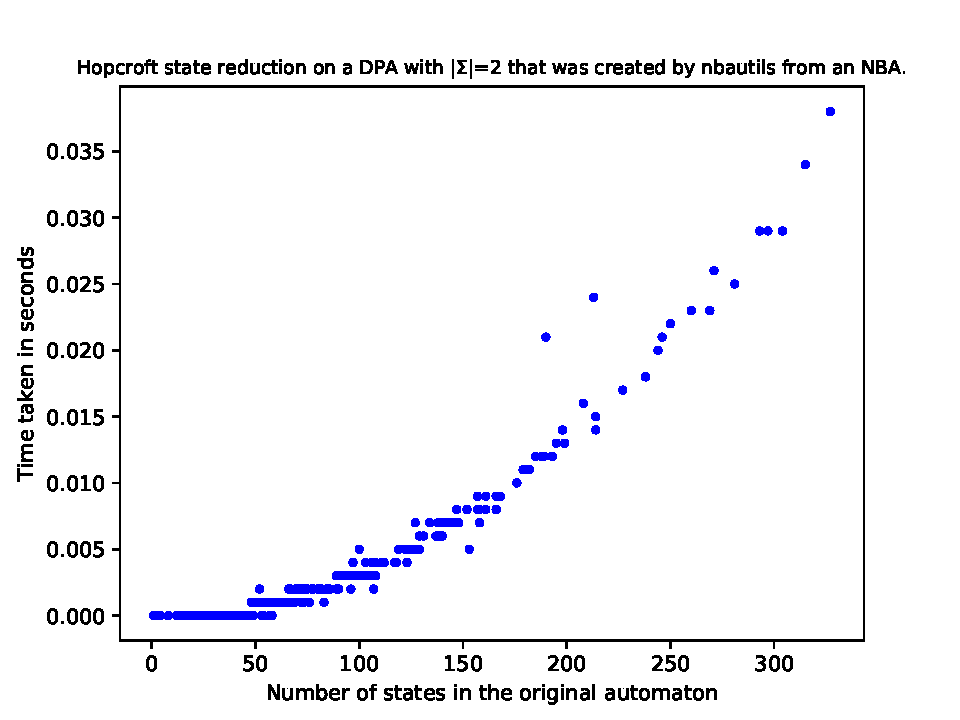
\includegraphics[page=1,height=.3\textheight]{../data/analysis/hopcroft/detnbaut_ap1.pdf} 
		\caption{Time of the state reduction of different automata using $\mu_M$.}
		\label{fig:general:empirical_moore_time}
	\end{minipage}
\end{figure}

\begin{figure}
	\centering
	\includegraphics[page=2,height=.4\textheight]{../data/analysis/hopcroft/detspot_ap1.pdf} 
	\caption{State reduction of \textsf{detspot} automata using $\mu_M$.}
	\label{fig:general:empirical_moore_reduct_abs}
\end{figure}



\vspace{5pt}





\section{Reachability}

\begin{defn}
	Let $\mathcal{S} = (Q, \Sigma, \delta)$ be a deterministic transition structure. We define the \emph{reachability order} $\preceq_\text{reach}^\mathcal{S}$ as $p \preceq_\text{reach}^\mathcal{S} q$ if and only if $q$ is reachable from $p$. 
\end{defn}

We want to note here that we always assume for all automata to only have one connected component, i.e. for all states $p$ and $q$, there is a state $r$ such that $p$ and $q$ are both reachable from $r$. In practice, most automata have an predefined initial state and a simple depth first search can be used to eliminate all unreachable states.

\begin{lem}
	$\preceq_\text{reach}^\mathcal{S}$ is a preorder.
\end{lem}

\begin{defn}
	Let $\mathcal{S} = (Q, \Sigma, \delta)$ be a deterministic transition structure. We call a relation $\preceq$ a \emph{total extension of reachability} if it is a minimal superset of $\preceq_\text{reach}^\mathcal{S}$ that is also a total preorder.
	
	For $p \preceq q$ and $q \preceq p$, we write $p \simeq q$.
\end{defn}

\begin{lem}
	For a given deterministic transition structure $\mathcal{S}$, a total extension of reachability is computable in $\mathcal{O}(|\mathcal{S}|)$.
	\label{lem:general:reach_topo_lintime}
\end{lem}

\begin{proof}
	Using e.g. Kosaraju's algorithm \cite{Sharir81}, the SCCs of $\mathcal{A}$ can be computed in linear time. We can now build a DAG from $\mathcal{A}$ by merging all states in an SCC into a single state; iterate over all transitions $(p, a, q)$ and add an $a$-transition from the merged representative of $p$ to that of $q$. Assuming efficient data structures for the computed SCCs, this DAG can be computed in $O(|\mathcal{A}|)$ time.
	
	To finish the computation of $\preceq$, we look for a topological order on that DAG. This is a total preorder on the SCCs that is compatible with reachability. All that is left to be done is to extend that order to all states.
\end{proof}




\section{Changing Priorities}
As we mentioned earlier, state reduction of DPAs is difficult and minimization is an NP-hard problem. Priorities of states on the other hand are generally easier to modify. A few of these possibilities are considered in this section.

\begin{lem}
\label{lem:general:trivial_scc_dont_matter}
	Let $\mathcal{A} = (Q, \Sigma, \delta, c)$ be a DPA and let $\{s\} \subseteq Q$ be a trivial SCC in $\mathcal{A}$. Let $\mathcal{A}' = (Q, \Sigma, \delta, c')$ be a copy of $\mathcal{A}$ with the only exception that $c'(s) = k$ for some arbitrary $k$. Then $\mathcal{A} \equiv_L \mathcal{A}'$.
\end{lem}

\begin{proof}
	Let $q \in Q$ be any state. We show that $L(\mathcal{A}, q) = L(\mathcal{A}', q)$. Let $\rho$ and $\rho'$ be the runs of $\mathcal{A}$ and $\mathcal{A}'$ starting in $q$ on some $\alpha \in \Sigma^\omega$. As $s$ lies in a trivial SCC, the runs visit that state at most once. Therefore, $\text{Inf} c(\rho) = \text{Inf} c'(\rho')$ and the runs have the same acceptance.
\end{proof}

\vspace{10pt}

An interesting property that parity automata can have is being \emph{normalized}. Even more important is that a normalized version of a DPA can be computed rather easily.

\begin{defn}
	Let $\mathcal{A} = (Q, \Sigma, \delta, c)$ be a DPA. We call $\mathcal{A}$ \emph{$c$-normalized} if for every state $q \in Q$ that does not lie in a trivial SCC and all priorities $k \leq c(q)$, there is a path from $q$ to $q$ such that the lowest priority visited is $k$.
\end{defn}


Algorithm \ref{alg:general:normalize_c} shows how an equivalent normalized priority function can be computed in $\mathcal{O}(|Q| \cdot |c(Q)|)$. The algorithm is a slight adaption of that presented in \cite{CartonMaceiras99}, which is why we will not go into further details here and just refer to the original source.

\begin{algorithm}[h!]
  \caption{Normalizing the priority function of a DPA.}
  \label{alg:general:normalize_c}
  \begin{algorithmic}[1]
    \Function{Normalize}{$\mathcal{A}$}
      \State $c' : Q \rightarrow \mathbb{N}, q \mapsto c(q)$
      \State \Call{M}{$\mathcal{A}$, $c'$}
      \State \Return{$c'$}
    \EndFunction
    \Statex
    \Function{M}{$\mathcal{A} \upharpoonright_P$, $c'$}
      \If{$P = \emptyset$}
        \State \Return 0
      \EndIf
      \State $min \gets 0$
      \For{SCC $S$ in $\mathcal{A} \upharpoonright_P$}
        \State $m := \min c(S) \mod 2$
        \State $X := c^{-1}(m)$
        \For{$q \in X$}
          \State $c'(q) \gets m$
        \EndFor
        \State $S' := S \setminus X$
        \State $m' \gets $\Call{M}{$\mathcal{A} \upharpoonright_{S'}$, $c'$}
        \If{$m'$ even}
          \If{$m$ even}
            \State $\delta := m$
          \Else
            \State $\delta := m-2$
          \EndIf
        \Else
          \State $\delta := m-1$
        \EndIf
        \For{$q \in S'$}
          \State $c'(q) \gets c'(q) - \delta$
        \EndFor
        \State $min \gets \min \{min, m\}$
      \EndFor
      \State \Return{$min$}
    \EndFunction
  \end{algorithmic}
\end{algorithm}











%
\section{Skip Merger}

The skip merger is the first reduction algorithm we want to introduce. It can be seen more of a first proof of concept rather than a practical novelty, as the underlying idea is neither complex nor had it great effect during empirical tests.

The skip merger considers the different strongly connected components (SCCs) of the automaton. An SCC is a set of states in which each element can reach every other via some path. We sometimes speak of the \enquote{deepest} SCCs with a certain property, which are those SCCs such that no other SCC with that property is reachable anymore.

If we have an equivalence relation that implies language equivalence but is not strong enough to warrant a merge of states on its own, each equivalence class of that relation only requires its states in the deepest SCC. We can therefore redirect any transition that would move the automaton to a state to a representative in a deepest SCC instead.

To formally capture this idea, the \emph{reachability preorder} is defined as $p \preceq_\text{reach} q$ if and only if $q$ is reachable by some path from $p$. Reachability can be computed in $\mathcal{O}(|Q|^3)$ which, in general, is too high of a complexity to efficiently deal with. It is sufficient to use a total extension of reachability though, which is a minimal superset of the reachability preorder that is a total preorder itself. Such a relation can be computed in linear time by a topological sorting on the SCCs of the automaton.

\begin{definition}
	Let $\sim$ be a congruence relation on $Q$. Let $\preceq$ be a total extension of reachability. For each $\kappa \in \mathfrak{C}$, we define $C_\kappa \subseteq \kappa$ to be the set of $\preceq$-maximal states and $M_\kappa = \kappa \setminus C_\kappa$.
		
	We define the \emph{skip merger function} $\mu_\text{skip}^\sim : \{ M_\kappa \mid \kappa \in \mathfrak{C}(\sim) \} \rightarrow 2^Q$ with $\mu_\text{skip}^\sim(M_\kappa) = C_\kappa$.
\end{definition}

\begin{theorem}
	If $\sim$ implies language equivalence, then a representative merge of a DPA w.r.t.\ $\mu_\text{skip}^\sim$ is language equivalent to the original.
\end{theorem}

\begin{proof}
	If we have two runs, $\pi$ and $\rho$, of the original DPA and the merged DPA on the same word $\alpha$, we can observe that at every position, $\pi(i)$ and $\rho(i)$ will be $\sim$-equivalent, as $\sim$ is a congruence relation. Furthermore, as there are only finitely many SCCs in an automaton, $\rho$ will eventually reach a point $j$ from which on only transitions are taken that also exist in the original DPA. As $\pi(j) \sim \rho(j)$, that means that the two runs must have the same status of acceptance. \qed
\end{proof}

\begin{theorem}
	For a given $\sim$ in a suitable data structure, $\mu_\text{skip}^\sim$ can be computed in $\mathcal{O}(|Q|)$.
\end{theorem}




\section{Fritz \& Wilke}
\label{sect:fritzwilke}

\subsection{Delayed Simulation Game}
In this section we consider delayed simulation games and variants thereof on DPAs. This approach is based on the paper \cite{FritzWilke06}, which considered the games for alternating parity automata. The DPAs we use are a special case of these APAs and therefore worth examining.

\begin{defn}
	For convenience, we define two orders for this chapter. First, we introduce $\checkmark$ as an \enquote{infinity} to the natural numbers and define the \textbf{obligation order} $\leq_\checkmark \subseteq (\mathbb{N} \cup \{\checkmark\}) \times (\mathbb{N} \cup \{\checkmark\})$ as $0 \leq_\checkmark 1 \leq_\checkmark 2 \leq_\checkmark \dots \leq_\checkmark \checkmark$.
	
	Second, we define an order of \enquote{goodness} on parity priorities $\preceq_\text{p} \subseteq \mathbb{N} \times \mathbb{N}$ as $0 \preceq_\text{p} 2 \preceq_\text{p} 4 \preceq_\text{p} \dots \preceq_\text{p} 5 \preceq_\text{p} 3 \preceq_\text{p} 1$.
\end{defn}

\begin{defn}
	Let $\mathcal{A} = (Q, \Sigma, \delta, c)$ be a DPA. We define the \emph{delayed simulation automaton} $\mathcal{A}_\text{de}(p, q) = (Q_\text{de}, \Sigma, \delta_\text{de}, F_\text{de})$ with starting state $q_0^\text{de}(p, q) = (p, q, \gamma(c(p), c(q), \checkmark))$, which is a deterministic Büchi automaton, as follows.
	
	\begin{itemize}
		\item $Q_\text{de} = Q \times Q \times (\text{img}(c) \cup \{ \checkmark \})$, i.e. the states are given as triples in which the first two components are states from $\mathcal{A}$ and the third component is either a priority from $\mathcal{A}$ or $\checkmark$.
		\item The alphabet remains $\Sigma$.
		\item $\delta_\text{de}( (p, q, k), a ) = ( p', q', \gamma(c(p'), c(q'), k)$, where $p' = \delta(p, a)$, $q' = \delta(q, a)$, and $\gamma$ is the same function as used in the initial state. The first two components behave like a regular product automaton.
		\item $F_\text{de} = Q \times Q \times \{ \checkmark \}$.
		\item The starting state is a triple $(p, q, \gamma(c(p), c(q), \checkmark))$, where $p, q \in Q$ are parameters given to the automaton, and $\gamma$ is defined below.
	\end{itemize}
	
	$\gamma : \mathbb{N} \times \mathbb{N} \times (\mathbb{N} \cup \{\checkmark\}) \rightarrow \mathbb{N} \cup \{\checkmark\}$ is the update function of the third component and defines the \enquote{obligations} as they are called in \cite{}. It is defined as 
	$$ \gamma(i, j, k) = \begin{cases}
		\checkmark & \text{if } i \text{ is odd and } i \leq_\checkmark k \text{ and } j \preceq_\text{p} i \\
		\checkmark & \text{if } j \text{ is even and } j \leq_\checkmark k \text{ and } j \preceq_\text{p} i \\
		\min_{\leq_\checkmark} \{ i,j,k \} & \text{else}
	\end{cases} $$
\end{defn}


\begin{defn}
	Let $\mathcal{A}$ be a DPA and let $\mathcal{A}_\text{de}$ be the delayed simulation automaton of $\mathcal{A}$. We say that a state $p$ $de$-simulates a state $q$ if $L(\mathcal{A}_\text{de}(p, q), q_0^\text{de}(p, q)) = \Sigma^\omega$. In that case we write $p \leq_\text{de} q$. If also $q \leq_\text{de} p$ holds, we write $p \equiv_\text{de} q$.
\end{defn}



\vspace{1cm}
\subsubsection*{$\boldsymbol{\equiv_\text{de}}$ is a congruence relation.}
Our overall goal is to use $\equiv_\text{de}$ to build a quotient automaton of our original DPA. The first step towards this goal is to show that the result is actually a well-defined DPA, by proving that the relation is a congruence.

\begin{lem}
\label{lem:fritzwilke:gamma_mono}
	$\gamma$ is monotonous in the third component, i.e. if $k \leq_\checkmark k'$, then $\gamma(i, j, k) \leq_\checkmark \gamma(i, j, k')$ for all $i, j \in \mathbb{N}$.
\end{lem}

\begin{proof}
	We consider each case in the definition of $\gamma$. If $i$ is odd, $i \leq_\checkmark k$ and $j \preceq_\text{p} i$, then also $i \leq_\checkmark k'$ and $\gamma(i, j, k) = \gamma(i, j, k') = \checkmark$.
	
	If $j$ is even, $j \leq_\checkmark k$ and $j \preceq_\text{p} i$, then also $j \leq_\checkmark k'$ and $\gamma(i, j, k) = \gamma(i, j, k') = \checkmark$.
	
	Otherwise, $\gamma(i, j, k) = \min \{i, j, k\}$ and $\gamma(i, j, k') = \min \{i, j, k'\}$. Since $k \leq_\checkmark k'$, $\gamma(i, j, k) \leq_\checkmark \gamma(i, j, k')$.
\end{proof}

\begin{lem}
\label{lem:fritzwilke:gamma_mono_ext}
	Let $\mathcal{A}$ be a DPA and let $p, q \in Q$, $k \in \mathbb{N} \cup \{\checkmark\}$. If the run of $\mathcal{A}_\text{de}$ starting at $(p, q, k)$ on some $\alpha \in \Sigma^\omega$ is accepting, then for all $k \leq_\checkmark k'$ also the run of $\mathcal{A}_\text{de}$ starting at $(p, q, k')$ on $\alpha$ is accepting.
\end{lem}

\begin{proof}
	Let $\rho$ be the run starting at $(p, q, k)$ and let $\rho'$ be the run starting at $(p, q, k')$. Further, let $p_i$, $q_i$, $k_i$, and $k'_i$ be the components of the states of those runs in the $i$-th step. Via induction we show that $k_i \leq_\checkmark k'_i$ for all $i$. Since $k_i$ is $\checkmark$ infinitely often, the same must be true for $k'_i$ and $\rho'$ is accepting.
	
	For $i = 0$, we have $k_0 = k \leq_\checkmark k' = k'_0$. Otherwise, we have $k_{i+1} = \gamma(c(p_{i+1}), c(q_{i+1}), k_i)$ and $k'_{i+1}$ analogously. The rest follows from Lemma \ref{lem:fritzwilke:gamma_mono}.
\end{proof}

\begin{lem}
\label{lem:fritzwilke:k_shrink}
	Let $\mathcal{A}$ be a DPA and $\rho \in Q_\text{de}^\omega$ be a run of $\mathcal{A}_\text{de}$ on some word. Let $k \in (\mathbb{N} \cup \{\checkmark\})^\omega$ be the third component during $\rho$. For all $i$, $k(i+1) \leq_\checkmark k(i)$ or $k(i+1) = \checkmark$.
\end{lem}

\begin{proof}
	Follows directly from the definition of $\gamma$.
\end{proof}

\begin{lem}
\label{lem:fritzwilke:n0_exists}
	Let $\mathcal{A}$ be a DPA with states $p, q \in Q$. For a word $\alpha \in \Sigma^\omega$, let $\rho : i \mapsto (p_i, q_i, k_i)$ be the run of $\mathcal{A}_\text{de}(p, q)$ on $\alpha$. If $\rho$ is not accepting, there is a position $n$ such that
	\begin{itemize}
		\item $\text{Occ}(\{p_i \mid i \geq n\}) = \text{Inf}(\{p_i \mid i \in \mathbb{N}\})$,
		\item $\text{Occ}(\{q_i \mid i \geq n\}) = \text{Inf}(\{q_i \mid i \in \mathbb{N}\})$,
		\item For all $i \geq j \geq n$, $k_i = k_j$ and $k_i \neq \checkmark$.
	\end{itemize}
	
	In other words, from $n$ on, $p$ and $q$ only see states that are seen infinitely often, and the obligations of $\rho$ do not change anymore.
\end{lem}

\begin{proof}
	The first two requirements are clear. Since states not in $\text{Inf}(\{p_i \mid i \in \mathbb{N}\})$ only occur finitely often, there must be positions $n_p$ and $n_q$ from which on they do not occur anymore at all.
	
	For the third requirement, we know that from some point on, the obligations $k$ never become $\checkmark$ anymore, as the run would be accepting otherwise. By Lemma \ref{lem:fritzwilke:k_shrink}, $k$ can only become lower from there on. As $\leq_\checkmark$ is a well-ordering, a minimum must be reached at some point $n_k$.
	
	The position $n_0 = \max \{n_p, n_q, n_k\}$ satisfies the statement.
\end{proof}

\begin{lem}
\label{lem:fritzwilke:run_goodness_implies_de}
	Let $\mathcal{A}$ be a DPA with two states $p, q \in Q$. Let $\alpha \in \Sigma^\omega$ be an $\omega$-word and let $\rho_p$ and $\rho_q$ be the respective runs of $\mathcal{A}$ on $\alpha$ starting in $p$ and $q$. If $\min \text{Inf}(c(\rho_q)) \preceq_p \min \text{Inf}(c(\rho_p))$, then $\alpha \in L(\mathcal{A}_\text{de}(p, q))$.
\end{lem}

\begin{proof}
	We write $l_q = \min \text{Inf}(c(\rho_q))$ and $l_p = \min \text{Inf}(c(\rho_p))$. Assume that the Lemma is false, so $l_q \preceq_p l_p$ but $\alpha \notin L(\mathcal{A}_\text{de}(p, q))$. Let $k_{13} \in (\mathbb{N} \cup \{\checkmark\})^\omega$ be the third component of the run of $\mathcal{A}_\text{de}(p, q)$ on $\alpha$. Let $n_0$ be a position as described in Lemma \ref{lem:fritzwilke:n0_exists} (for $\rho$). 
	
	\paragraph{Case 1: $l_q$ is even and $l_q \leq l_p$} We know $k_{13}(n_0) = l_q$, as that is the smaller value. Let $m > n_0$ be a position with $c(\rho_q(m)) = l_q$. Then $c(\rho_q(m))$ is even and $c(\rho_q(m)) = l_q \leq l_p \leq c(\rho_p(m))$, so $c(\rho_q(m)) \preceq_p c(\rho_p(m))$. Also we have $c(\rho_q(m)) \leq k_{13}(m-1) = l_q$ and therefore $k_{13}(m) = \checkmark$, which contradicts the choice of $n_0$.
	
	\paragraph{Case 2: $l_p$ is odd and $l_q \geq l_p$} We know $k_{13}(n_0) = l_p$. Let $m > n_0$ be a position with $c(\rho_p(m)) = l_p$. Then $c(\rho_p(m))$ is odd and $c(\rho_p(m)) = l_p \leq l_q \leq c(\rho_q(m))$, so $c(\rho_q(m)) \preceq_p c(\rho_p(m))$. By the same argumentation as above, we deduce $k_{13}(m) = \checkmark$.
\end{proof}

\begin{lem}
\label{lem:fritzwilke:de_order_reftran}
	Let $\mathcal{A}$ be a DPA. Then $\leq_\text{de}$ is reflexive and transitive.
\end{lem}

\begin{proof}
	For reflexivitiy, we need to show that $q \leq_\text{de} q$ for all states $q$. This is rather easy to see. For a word $\alpha \in \Sigma^\omega$, the third component of states in the run of $\mathcal{A}_\text{de}(q, q)$ on $\alpha$ is always $\checkmark$, as $\gamma(i, i, \checkmark) = \checkmark$.
	
	For transitivity, let $q_1 \leq_\text{de} q_2$ and $q_2 \leq_\text{de} q_3$. Assume towards a contradiction that $q_1 \not\leq_\text{de} q_3$, so there is a word $\alpha \notin L(\mathcal{A}_\text{de}(q_1, q_3))$. We consider the three runs $\rho_{12}$, $\rho_{23}$, and $\rho_{13}$ of $\mathcal{A}_\text{de}(q_1, q_2)$, $\mathcal{A}_\text{de}(q_2, q_3)$, and $\mathcal{A}_\text{de}(q_1, q_3)$ respectively on $\alpha$. Then $\rho_{12}$ and $\rho_{23}$ are accepting, whereas $\rho_{13}$ is not. 
	
	Moreover, we use the notation $q_1(i), q_2(i), q_3(i)$ for the states of the run and $k_{12}(i), k_{23}(i), k_{13}(i)$ for the obligations. More specifically for a run $\rho_{ij}$, it is true that $\rho_{ij}(n) = (q_i(n), q_j(n), k_{ij}(n))$.
	
	Let $n_0$ be a position as described in Lemma \ref{lem:fritzwilke:n0_exists} (for $\rho_{13}$) and let $l_j = \min \{ c(q_j(i)) \mid i \geq n_0 \}$ be the lowest priority that $q_j$ reaches after $n_0$.	This is equivalent to $l_j = \min \text{Inf}(\{ c(q_j(i)) \mid i \in \mathbb{N}\})$. We now show that $l_3 \preceq_p l_1$. By Lemma \ref{lem:fritzwilke:run_goodness_implies_de} this gives us $\alpha \in L(\mathcal{A}_\text{de}(q_1, q_3))$, letting us conclude in a contradiction.
	
	\paragraph{Case 1: $l_2$ is even.} We claim that $l_3$ is even and $l_3 \leq l_2$. 
	
	First, to show $l_3 \leq l_2$, let $m \geq n_0$ be a position with $c(q_2(m)) = l_2$ and let $n \geq m$ be the minimal position with $k_{23}(n) = \checkmark$. If $m = n$, then $c(q_3(n)) \preceq_p c(q_2(n)) = l_2$ and therefore $c(q_3(n)) \leq l_2$. Otherwise, from $m$ to $n-1$, $k_{23}$ only grows smaller and is at most $l_2$ (Lemma \ref{lem:fritzwilke:k_shrink}). As the priority of $q_2$ never becomes an odd number smaller than $l_2$, the only way for $k_{23}(m)$ to be $\checkmark$ is that $c(q_3(m))$ is even and $c(q_3(m)) \leq k_{23}(m-1) \leq l_2$.
	
	Second, assume that $l_3$ is odd and let $m$ be a position with $c(q_3(m)) = l_3$. As $l_2$ is even, we have $k_{23}(m) \leq l_3 < l_2$. At no future position can $c(q_3)$ both be even and smaller than $k_{23}$, so $k_{23}$ never becomes $\checkmark$ again. Thus, $\rho_{23}$ is not accepting.
	
	We claim that $l_1$ is odd or $l_1 \geq l_2$.
	
	Towards a contradiction assume the opposite, so $l_1 < l_2$ and $l_1$ is even. Let $m \geq n_0$ be a position with $c(q_1(m)) = l_1$. Then $c(q_2(m)) \not\preceq_p c(q_1(m))$ and therefore $k_{12}(m) = l_1$. At no position after $m$ can it happen that the conditions for $k_{12}$ to become $\checkmark$ again are satisfied. Thus, $\rho_{12}$ would not be accepting.
	
	If $l_1$ is odd and $l_3$ is even, $l_3 \preceq_p l_1$ follows. For the other case, $l_1$ and $l_3$ both being even with $l_3 \leq l_2 \leq l_1$, that also holds.
	
	\paragraph{Case 2: $l_2$ is odd.} We skip the details of this case as it works symmetrically to case 1. In particular, we first show that $l_1$ is odd and $l_1 \leq l_2$. We continue with $l_3$ being even or $l_3 \geq l_2$. From these two statements, $l_3 \preceq_p l_1$ again follows.
\end{proof}

\begin{theorem}
	Let $\mathcal{A}$ be a DPA. Then $\equiv_\text{de}$ is a congruence relation.
\end{theorem}

\begin{proof}
	The three properties that are required for $\equiv_\text{de}$ to be a equivalence relation are rather easy to see. Reflexivity and transitivity have been shown for $\leq_\text{de}$ already and symmetry follows from the definition. Congruence requires more elaboration.

	Let $p \equiv_\text{de} q$ be two equivalent states. Let $a \in \Sigma$ and $p' = \delta(p, a)$ and $q' = \delta(q, a)$. We have to show that also $p' \equiv_\text{de} q'$. Towards a contradiction, assume that $p' \not\leq_\text{de} q'$, so there is a word $\alpha \notin L(\mathcal{A}_\text{de}(p', q'))$. Let $(p', q', k) = \delta_\text{de}((p, q, \checkmark), a)$. By Lemma \ref{lem:fritzwilke:gamma_mono_ext}, the run of $\mathcal{A}_\text{de}$ on $\alpha$ from $(p', q', k)$ cannot be accepting; otherwise, the run of $\mathcal{A}_\text{de}$ from $(p', q', \checkmark)$ would be accepting and $\alpha \in L(\mathcal{A}_\text{de}(p', q'))$. Hence, $a \alpha \notin L(\mathcal{A}_\text{de}(p, q))$, which means that $p \not\equiv_\text{de} q$.
\end{proof}

We want to mention here that $\equiv_\text{de}$ is actually an equivalence relation on APAs as well, as was shown in the original paper. However, congruence is the key point at which deterministic automata diverge. Congruence requires something to be true for \emph{all} successors of a state; delayed simulation only requires there to be \emph{one} equivalent pair of successors. Only in deterministic automata is it that these two coincide.



\vspace{1cm}
\subsubsection*{Alternative characterization}
Having described several properties of $\leq_\text{de}$ and $\equiv_\text{de}$ in the previous part, we briefly want to give an alternative description in corollary \ref{cor:fritzwilke:equivde_alternative} of what it means for two states to be de-simulation equivalent. The intention is to give a more intuitive understanding as well as provide a framework to make future proofs more comfortable.

\begin{lem}
\label{lem:fritzwilke:preceq_alternative}
	Let $\mathcal{A}$ be a DPA with states $p, q \in Q$. Then $p \preceq_\text{de} q$ if and only if the following property holds for all $w \in \Sigma^*$: 
	
	Let $p' = \delta^*(p, w)$ and $q' = \delta^*(q, w)$. If $c(p')$ is even and $c(p') < c(q')$, then every path from $q'$ eventually reaches a priority at most $c(p')$. On the other hand, if $c(q')$ is odd and $c(q') < c(p')$, then every path from $p'$ eventually reaches a priority at most $c(q')$.
\end{lem}

\begin{proof}
	\textbf{If} We show the contrapositive. Let $p \not\preceq_\text{de} q$, so there is a word $\alpha \notin L(\mathcal{A}_\text{de}(p, q))$ with the run of $\mathcal{A}_\text{de}(p, q)$ being $(p_0, q_0, k_0) (p_1, q_1, k_1) \dots$. By Lemma \ref{lem:fritzwilke:n0_exists}, there is a position $n$ such that $k_i$ does not change anymore for $i \geq n$. We define $w = \alpha[0, n_0]$ and $\beta = \alpha[n_0+1, ]$ (so $\alpha = w\beta$) and claim that $w$ is a valid counterexample for the right-side property.
	
	The first case is: $c(p') < c(q')$ and $c(p')$ is even. \\
	Reading $\beta$ from $q'$ induces a run that never visits a priority less or equal to $c(p')$: Let $u \sqsubset \beta$ and assume that $c(\delta^*(q', u)) \leq c(p')$. By choice of $n$, we know that $k_{|wu|} = k_{|wu|+1} \neq \checkmark$. This can only happen if the \enquote{else} case of $\gamma$ is hit, meaning that $k_{|wu|+1} = \min \{ k_{|wu|}, c(\delta^*(p', u)), c(\delta^*(q', u)) \}$. Specifically, $c(\delta^*(q', u)) \geq k_{|wu|}$. By choice of $w$ we also have $k_{|wu|} = k_{|w|} \leq c(p')$, so $c(\delta^*(q', u)) = c(p')$.
	
	This, however, means that $c(\delta^*(q', u))$ is even, $c(\delta^*(q', u)) \leq_\checkmark k_{|wu|}$, and $c(\delta^*(q', u)) \preceq_p c(p')$ and thus $k_{|wu|+1} = \checkmark$ which is a contradiction.
	
	The second case, $c(q') < c(p')$ and $c(q')$ is odd, works almost identically so we omit the proof here.
	
	\paragraph{Only If} Again we show the contrapositive: There is a $w \in \Sigma^*$ such that the right-side property is violated. Let this $w$ now be chosen among all these words such that $\min \{ c(p'), c(q') \}$ becomes minimal. We now show that $p \not\preceq_\text{de} q$. 
	
	The first case is: $c(p') < c(q')$ and $c(p')$ is even. \\
	Let $\beta \in \Sigma^\omega$ be a word such that the respective run from $q'$ only sees priorities strictly greater than $c(p')$. Let $(p_0, q_0, k_0) (p_1, q_1, k_1) \dots$ be the run of $\mathcal{A}_\text{de}(p, q)$ on $\alpha = w \beta$. We claim that $k_i \neq \checkmark$ for all $i > |w|$. If that is true, then the run is rejecting and $\alpha \notin L(\mathcal{A}_\text{de}(p, q))$.
	
	Assume towards a contradiction that $k_i$ does become $\checkmark$ again at some point. Let $j \geq |w|$ be the minimal position with $k_{j+1} = \checkmark$. Then by definition of $\gamma$, $c(q_{j+1}) \leq k_j$ is even or $c(p_{j+1}) \leq k_j$ is odd. In the former case, we would have a contradiction to the choice of $\beta$. In the latter case, we would have a contradiction to the choice of $w$ as a word with minimal priority at $c(p')$: since $c(p')$ is even, $c(p_{j+1}) < c(p')$ and from $q_{j+1}$ there is a run that never reaches a smaller priority. Hence, $w \cdot \beta[0, j-|w|]$ would have been our choice for $w$ instead.
	
	The second case, $c(q') < c(p')$ and $c(q')$ is odd, works almost identically so we omit the proof here.
\end{proof}

While this characterization of $\preceq_\text{de}$ seems arbitrary, it allows for an easier definition of $\equiv_\text{de}$ as is seen in the following statement.

\begin{cor}
\label{cor:fritzwilke:equivde_alternative}
	Let $\mathcal{A}$ be a DPA with states $p, q \in Q$. Then $p \equiv_\text{de} q$ if and only if the following holds for all words $w \in \Sigma^*$:
	
	Let $p' = \delta^*(p, w)$ and $q' = \delta^*(q, w)$. Every run that starts in $p'$ or $q'$ eventually sees a priority less than or equal to $\min \{c(p'), c(q')\}$.
\end{cor}



\vspace{1cm}
\subsubsection*{Using delayed simulation as a merger}
In general, delayed simulation does not imply equal priorities. It is not obvious if a quotient automaton can be built by choosing an arbitrary representative of each equivalence class and in fact example %TODO
shows that this is not the case. However, the following theorem solves this issue.

\begin{lem}
\label{lem:fritzwilke:equiv_states_same_minpri}
	Let $\mathcal{A}$ be a DPA and let $\pi$ and $\rho$ be runs of $\mathcal{A}$ on the same word $\alpha$ but starting at different states. If $\pi(0) \equiv_\text{de} \rho(0)$, then $\min \text{Occ}(c(\pi)) = \min \text{Occ}(c(\rho))$.
\end{lem}

\begin{proof}
	Let $\pi(0) = p$ and $\rho(0) = q$. Assume towards a contradiction that $\min \text{Occ}(c(\pi)) < \min \text{Occ}(c(\rho))$. Let $k = \min \text{Occ}(c(\pi))$ and let $n$ be the first position at which $c(\pi(n)) = k$. Let $p' = \pi(n)$ and $q' = \rho(n)$. These two states are reachable from $p$ and $q$ respectively with the word $\alpha[0,n]$.
	
	By Corollary \ref{cor:fritzwilke:equivde_alternative}, the run $\rho[n,\omega]$ must eventually see a priority at most $k$ which contradicts the assumption.
\end{proof}


\begin{theorem} 
\label{thm:fritzwilke:combine_priorities}
	Let $\mathcal{A} = (Q, \Sigma, \delta, c)$ be a DPA and let $p, q \in Q$ with $p \equiv_\text{de} q$ and $c(p) < c(q)$. Define $\mathcal{A}' = (Q, \Sigma, \delta, c')$ with $c'(s) = \begin{cases} c(p) & \text{if } s = q \\ c(s) & \text{else} \end{cases}$. Then $\mathcal{A} \equiv_L \mathcal{A}'$.
\end{theorem}

\begin{proof}
	Let $q_0 \in Q$ be an arbitrary state. We show that $L(\mathcal{A}, q_0) = L(\mathcal{A}', q_0)$.
	
	First, consider the case that $c(p)$ is an even number. The parity of each state is at least as good in $\mathcal{A}'$ as it is in $\mathcal{A}$, so $L(\mathcal{A}, q_0) \subseteq L(\mathcal{A}', q_0)$. For the other direction, assume there is an $\alpha \in L(\mathcal{A}', q_0) \setminus L(\mathcal{A}, q_0)$, so the respective run $\rho \in Q^\omega$ is accepting in $\mathcal{A}'$ but not in $\mathcal{A}$. 
	
	For this to be true, $\rho$ must visit $q$ infinitely often and $c'(q)$ must be the lowest priority that occurs infinitely often; otherwise, the run would have the same acceptance in both automata. Thus, there is a finite word $w \in \Sigma^*$ such that from $q$, $\mathcal{A}$ reaches again $q$ via $w$ and inbetween only priorities greater than $c'(q)$ are seen.
	
	Now consider the word $w^\omega$ and the run $\pi_q$ of $\mathcal{A}$ on said word starting in $q$. With the argument above, we know that the minimal priority occuring in $c(\pi_q)$ is greater than $c'(q)$. If we take the run $\pi_p$ on $w^\omega$ starting at $p$ though, we find that this run sees priority $c(p) = c'(q)$ at the very beginning. This contradicts Lemma \ref{lem:fritzwilke:equiv_states_same_minpri}, as $p \equiv_\text{de} q$. Thus, the described $\alpha$ cannot exist. 
	
	If $c(p)$ is an odd number, a very similar argumentation can be applied with the roles of $\mathcal{A}$ and $\mathcal{A}'$ reversed. We omit this repetition.
\end{proof}

\vspace{5pt}

Together with Lemma \ref{lem:general:congrel_prio_implies_moore}, this allows for a merger function that preservers language.

\begin{defn}
	We define the \emph{delayed simulation merger} as $\mu_\text{de} : \mathfrak{C}(\equiv_\text{de}) \rightarrow 2^Q$ with $\mu_\text{de}(\kappa) = c^{-1}(\min c(\kappa))$.
\end{defn}

\begin{cor}
	Let $\mathcal{A}$ be a DPA. Then $\mathcal{A}$ is language equivalent to every representative merge w.r.t. $\mu_\text{de}$.
\end{cor}

\begin{proof}
	With Theorem \ref{thm:fritzwilke:combine_priorities}, we can construct a language equivalent $\mathcal{A}' = (Q, \Sigma, \delta, c')$ such that for all $\kappa \in \mathfrak{C}(\equiv_\text{de})$, all states in $\kappa$ have the same priority in $c'$. Every representative merge of $\mathcal{A}$ w.r.t. $\mu_\text{de}$ is a representative merge of $\mathcal{A}'$ w.r.t. $\mu_\text{de}$.
	
	In $\mathcal{A}'$, $\mu_\text{de}$ is the same as $\mu^{\equiv_\text{de}}_\div$. The fact that representative merges of $\mathcal{A}'$ w.r.t. $\mu_\text{de}$ preserve language follows from Lemma \ref{lem:general:congrel_prio_implies_moore}.
\end{proof}

\vspace{10pt}

Finally, we provide a quick analysis of the computational effort for delayed simulation.

\begin{theorem}
	For a given DPA $\mathcal{A}$, $\equiv_\text{de}$ can be computed in $\mathcal{O}(|Q|^2 \cdot |c(Q)|)$.
\end{theorem}

\begin{proof}
	$\mathcal{A}_\text{de}$ is of size $\mathcal{O}(|Q|^2 \cdot |c(Q)|)$. Building it is a straight-forward construction. Once the delayed simulation automaton is built, we have to solve the universal problem, i.e. find all states from which all words are accepted. For DBAs this can be done in linear time with depth search or similar algorithms.
\end{proof}






\vspace{10pt}

\subsubsection{Resetting obligations} 
In the delayed simulation automaton, \enquote{obligations} correspond to good priorities that the first state has accumulated or bad priorities that the second state has accumulated and the need for the respective other state to compensate in some way. The intuitive idea behind this concept is that an obligation that cannot be compensated, stands for an infinite run in which the acceptance differs between the two states that are being compared. The issue with the original definition is that obligations carry over, even if they can only be caused finitely often. This is demonstrated in figure \ref{fig:fritzwilke:reset_oblig_example}; the two states could be merged into one, but they are not $\equiv_\text{de}$-equivalent as can be seen in the delayed simulation automaton in figure \ref{fig:fritzwilke:reset_oblig_example_dea}.

\begin{figure}
\centering
\begin{tikzpicture}[shorten >=1pt,node distance=2cm,on grid,initial text=]
  \node[state,initial]   (0)                {0};
  \node[state]           (1) [right=of 0] {1};
  \path[->] (0) edge node [above] {a} (1)
            (1) edge [loop right] node {a} (1);
\end{tikzpicture}
\caption{Example automaton in which the states could be merged but delayed simulation separates them.}
\label{fig:fritzwilke:reset_oblig_example}
\end{figure}

\begin{figure}
\centering
\begin{tikzpicture}[shorten >=1pt,node distance=2cm,on grid,initial text=]
  \node[state]   (0)                {$0,1,0$};
  \node[state]   (1) [right=of 0] {$1,1,0$};
  \path[->] (0) edge node [above] {a} (1)
            (1) edge [loop right] node {a} (1);
\end{tikzpicture}
\caption{Delayed simulation automaton for \ref{fig:fritzwilke:reset_oblig_example}.}
\label{fig:fritzwilke:reset_oblig_example_dea}
\end{figure}

As a solution to this, we propose a simple change to the definition of the automaton which resets the obligations every time, either state moves to a new SCC. 

\begin{defn}
	Let $\mathcal{A} = (Q, \Sigma, q_0, \delta, c)$ be a DPA. We define the \emph{delayed simulation automaton with SCC resets} $\mathcal{A}_\text{deR}(p, q) = (Q_\text{de}, \Sigma, \delta_\text{deR}, F_\text{de})$ with $\delta_\text{deR}((p, q, k), a) = \delta_\text{de}((p, q, \text{reset}(p, q, k, a)), a)$. Except for the addition of the reset function, this automaton is the same as $\mathcal{A}_\text{de}$.
	
	If $p$ and $\delta(p, a)$ lie in the same SCC, as well as $q$ and $\delta(q, a)$, then we simply set $\text{reset}(p, q, k, a) =~k$. Otherwise, i.e. if any state changes its SCC, the reset comes into play and we set $\text{reset}(p, q, k, a) = \checkmark$.
	
	We write $p \leq_\text{deR} q$ if $L(\mathcal{A}_\text{deR}(p, q), q_0^\text{de}(p, q)) = \Sigma^\omega$. If also $q \leq_\text{deR} p$ holds, we write $p \equiv_\text{deR} q$.
\end{defn}

As the definition is so similar to the original delayed simulation, most results that we have already proven translate directly to the new relation. 

\begin{theorem}
	$\equiv_\text{deR}$ is a congruence relation.
\end{theorem}

\begin{lem}
	$\leq_\text{de} \;\subseteq\; \leq_\text{deR}$.
\end{lem}

\begin{proof} 
	Consider the two simulation automata $\mathcal{A}_\text{de}(p, q)$ and $\mathcal{A}_\text{deR}(p, q)$ and let $\alpha \in \Sigma^\omega$ be an arbitrary word. Let $(p_i, q_i, k_i)_{i \in \mathbb{N}}$ and $(p_i, q_i, l_i)_{i \in \mathbb{N}}$ be the runs of these two automata on $\alpha$. We claim that $k_i \leq_\checkmark l_i$ at every position. Then, since $L(\mathcal{A}_\text{de}(p, q), q_0^\text{de}(p, q)) = \Sigma^\omega$, both runs must be accepting.
	
	We know $k_0 = l_0$ by definition. For the sake of induction, we look at position $i+1$. If neither $p_i$ nor $q_i$ change their SCC in this step, the statement follows from lemma \ref{lem:fritzwilke:gamma_mono}. Otherwise, $l_{i+1} = \checkmark \geq_\checkmark k_{i+1}$.
\end{proof}

\vspace{5pt}

Unfortunately, Theorem \ref{thm:fritzwilke:combine_priorities} does not translate easily to $\equiv_\text{deR}$. In fact, we were not able to find a characterization for a merger function except for the option to only merge states within single SCCs. Then, however, using the skip merger in combination with normal delayed simulation yields a result just as good.























\section{Iterated Moore Equivalence}
\label{sect:imoore}

Standard Moore equivalence was created to minimize Moore automata in which the priority of every state matters; in other words, the occurrence set of a given run is considered. Parity automata on the other hand only use the smaller infinity set. The idea of the upcoming approach is to use this relaxation to give the standard Moore equivalence more freedom and remove additional states.

\begin{defn}
	Let $\mathcal{A} = (P, \Sigma, \delta, c)$ and $\mathcal{B} = (Q, \Sigma, \varepsilon, d)$ be DPAs and $S \subseteq P$. We say that \emph{$\mathcal{A}$ prepends $S$ to $\mathcal{B}$} if 
	\begin{itemize}
		\item $Q \cap S = \emptyset$
		\item $P = Q \cup S$
		\item $\delta\upharpoonright_{Q \times \Sigma} = \varepsilon$
		\item $c\upharpoonright_Q = d$
	\end{itemize}
	
	We assume $S$ to be an SCC in these use cases, i.e. from every $s \in S$, every other $s' \in S$ is reachable in $\mathcal{A}$.
\end{defn} 

\begin{defn}
\label{def:fwe:itmoore}
	Let $\mathcal{A} = (Q, \Sigma, \delta, c)$ be a DPA with SCCs $\mathcal{S} \subseteq 2^Q$. Let $\preceq \,\subseteq \mathcal{S} \times \mathcal{S}$ be a total preorder on the SCCs such that $S \preceq S'$ implies that $S'$ is reachable from $S$. For the $i$-th element w.r.t. this order, we write $S_i$, i.e. $S_0 \prec S_1 \prec \dots \prec S_{|\mathcal{S}|}$. 
	
	For every state $q$ in $\mathcal{A}$, let $\text{SCC}(q)$ be the SCC of $q$ and let $\text{SCCi}(q)$ be the index of that SCC, i.e. $\text{SCC}(q) = S_{\text{SCCi}(q)}$. Let $\preceq_Q \,\subseteq Q \times Q$ be a total preorder on the states such that $q \preceq_Q q'$ implies $\text{SCCi}(q) \leq \text{SCCi}(q')$.
	
	We inductively define a sequence of automata $(\mathcal{B}_i)_{0 \leq i \leq |\mathcal{S}|}$. For every $i$, we write $\mathcal{B}_i = (Q_i, \Sigma, \delta_i, c_i)$.
	
	\begin{itemize}
		\item The state sets are defined as $Q_i = \bigcup_{j=i}^{|\mathcal{S}|} S_j$.
		\item The base case is $\mathcal{B}_{|\mathcal{S}|} = \mathcal{A}\upharpoonright_{S_{|\mathcal{S}|}}$.
		\item Given that $\mathcal{B}_{i+1}$ is defined, let $\mathcal{B}'_i = (Q_i, \Sigma, q_0^{\prime i}, \delta_i, c'_i)$ be a DPA that prepends $S_i$ to $\mathcal{B}_{i+1}$ such that $\delta \upharpoonright_{Q_i \times \Sigma} = \delta_i$ and $c \upharpoonright_{S_i} = c'_i \upharpoonright_{S_i}$.
		\item Let $M'_i$ be the Moore equivalence on $\mathcal{B}'_i$. If $S_i = \{q\}$ is a trivial SCC, $q$ is not $M'_i$-equivalent to any other state, and there is a $p \in Q_{i+1}$ such that for all $a \in \Sigma$ $(\delta'_i(q, a), \delta'_i(p, a)) \in M'_i$, then let $p_0$ be $\preceq_Q$-maximal among those $p$ and let $c_i(r) = \begin{cases} c_{i+1}(p_0) & \text{if } r = q \\ c_{i+1}(r) & \text{else} \end{cases}$. If any of the three conditions is false, simply set $c_i = c'_i$.
	\end{itemize} 
	
	Let $M_i$ be the Moore equivalence on $\mathcal{B}_i$. We define $\equiv_{IM} \,:= M_0$ and call this the \emph{iterated Moore equivalence} of $\mathcal{A}$.
\end{defn}

At first, this definition might confuse when written down formally like this. %TODO example
We continuously add the SCCs of $\mathcal{A}$ starting from the \enquote{back}. In addition to computing the usual Moore equivalence on our automaton, we also take trivial SCCs into special consideration; as their priority cannot appear infinitely often on any run, its value is effectively arbitrary. We can therefore perform extra steps to more liberally merge it with other states.

In the upcoming statements we prove the important properties of iterated Moore equivalence.

\begin{lem}
\label{lem:itm:mset_stays_same}
	Let variables be as in definition \ref{def:fwe:itmoore}. For all $i$ and all $p, q \in Q_{i+1}$, $(p, q) \in M'_i$ iff $(p, q) \in M_{i+1}$. For all $i$ and all $p, q \in Q_{i+1}$, $(p, q) \in M_i$ iff $(p, q) \in M'_i$.
\end{lem}

\begin{proof}
	%TODO
\end{proof}

\begin{theorem}
	Let $\mathcal{A}$ be a DPA. Then $|\mathfrak{C}(\equiv_M)| \geq |\mathfrak{C}(\equiv_{IM})|$.
\end{theorem}

\begin{proof}
	We use induction as in the construction of $\equiv_{IM}$. For every $i$, let $\mathcal{A}_i = \mathcal{A} \upharpoonright_{Q_i}$ and let $N_i$ be the Moore equivalence in $\mathcal{A}_i$. Our goal is to prove $|\mathfrak{C}(N_0)| \geq |\mathfrak{C}(M_0)|$. For $i = |\mathcal{S}|$, $B_i = A_i$, so $|\mathfrak{C}(N_i)| = |\mathfrak{C}(M_i)|$ is trivial.
	
	Now assume that $|\mathfrak{C}(N_i)| \geq |\mathfrak{C}(M_i)|$ is given. By Lemma \ref{lem:itm:mset_stays_same}, we know $N_{i-1} \cap (Q_i \times Q_i) = N_i$ and $M_{i-1} \cap (Q_i \times Q_i) = M_i$, as no state in $S_{i-1}$ is reachable from any state in $Q_i$. Now assume that $|\mathfrak{C}(N_{i-1})| < |\mathfrak{C}(M_{i-1})|$, so there is at least one new equivalence class added to $M_{i-1}$ that was not added in $N_{i-1}$. In other words, if we call this class $\kappa$, then $\kappa \cap M_i = \emptyset$ but $\kappa \cap N_i \neq \emptyset$. 
	
	We consider two cases. First, if $c_{i-1} = c'_{i-1}$, let $p \in \kappa \cap N_i$ and $q \in \kappa \cap S_{i-1}$, so $(p, q) \in N_{i-1}$ but $(p, q) \notin M_{i-1}$. %TODO
\end{proof}


\newpage

\begin{theorem}
	Let variables be defined as in definition \ref{def:fwe:itmoore} and let $\sim_M$ be the Moore equivalence of $\mathcal{A}$. Then $\sim_M \,\subseteq\, \sim_{IM}$.
\end{theorem}

\begin{proof}
	Let $p, q$ be two states with $p \sim_M q$ but $p \not\sim_{IM} q$ such that $\max \{\text{SCCi}(p), \text{SCCi}(q)\}$ is maximal among all possible pairs; if there are multiple pairs with the highest value, choose a pair which has maximal $\min \{\text{SCCi}(p), \text{SCCi}(q)\}$ as well.
	
	Without loss of generality we can assume that $c_0(p) \neq c_0(q)$ as we can always find such a pair with the definition of Moore equivalence. Since $c(p) = c(q)$, at least one of the two states must have a different priority in $c_0$ compared to $c$. By symmetry, assume that state is $q$. $\{q\}$ must be a trivial SCC in $\mathcal{A}$. Let $q'$ be the $\preceq_Q$-maximal state s.t. $(\delta(q, a), \delta(q', a)) \in M'_{\text{SCCi}(q)}$ for all $a \in \Sigma$, that is the state whose priority was copied to $q$.
	
	We can make the assumption that $\text{SCCi}(q) > \text{SCCi}(p)$: if $c(p) \neq c_0(\text{SCCi}(p))$, then $\{p\}$ is a trivial SCC and the choice of the states is symmetric. Otherwise, if we would have $\text{SCCi}(p) > \text{SCCi}(q)$ and $c(p) = c_0(\text{SCCi}(p))$, then $(p, q) \in M_{\text{SCCi}(q)} \subseteq\, \sim_{IM}$. 
	
	Consider the case that $\text{SCC}(p)$ is a non-trivial SCC, so there is a non-empty word $w$ with $\delta^*(p, w) = p$. Because of the congruence property, we know $q \sim_M p \sim_M \delta^*(p, w) \sim_M \delta^*(q, w)$. As $\{q\}$ is a trivial SCC, $\text{SCCi}(\delta^*(q, w)) > \text{SCCi}(q)$. That means that every state that is $\sim_M$-equivalent to $\delta^*(q, w)$ must also be $\sim_{IM}$-equivalent to it; otherwise, the choice of $(p, q)$ as a pair with maximal value of $\text{SCCi}(q)$ would be contradicted. In particular, $q \sim_{IM} \delta(q, w) \sim_{IM} p$, which breaks our initial assumption.
	\vspace{5pt}
	
	Finally, we look at the case that $\text{SCC}(p) = \{p\}$ is trivial. First, if $c(p) \neq c_0(p)$, then there must be a state $p'$ s.t. $(\delta(p, a), \delta(p', a)) \in M'_{\text{SCCi}(p)}$ for all $a \in \Sigma$; consider the $\preceq_Q$-maximal state that satisfies this. We can show that $p'$ must be the same as $q'$ and therefore $c_0(p) = c_0(q') = c_0(q)$, which would be a contradiction. The only possibility for this to be false is that there is an $a \in \Sigma$ such that $(\delta(p, a), \delta(p', a)) \in M'_{\text{SCCi}(p)}$ but $(\delta(p, a), \delta(q', a)) \notin M'_{\text{SCCi}(p)}$. Remember that $(\delta(q, a), \delta(q', a)) \in M'_{\text{SCCi}(p)}$ and $\delta(q, a) \sim_M \delta(p, a)$. If now $(\delta(p, a), \delta(q', a)) \notin M'_{\text{SCCi}(p)}$ would hold, then $(\delta(p, a), \delta(q, a)) \notin M'_{\text{SCCi}(p)} \subseteq M_0$, so $\delta(p, a) \not\sim_{IM} \delta(q, a)$. Since $\{q\}$ is a trivial SCC, $\text{SCCi}(q) < \text{SCCi}(\delta(p, a))$, meaning that the pair $(\delta(p, a), \delta(q, a))$ would contradict our choice of $(p, q)$.
	
	Second, if $c(p) = c_0(p)$, then there must be a state $p' \neq p$ s.t. $(p, p') \in M'_{\text{SCCi}(p)} \subseteq M_0$. Let that $p'$ be $\preceq_Q$-maximal. $\text{SCC}(p')$ cannot be a trivial SCC: note that $q \sim_{IM} q'$ and $p \sim_{IM} p'$. Furthermore, $\delta(p, a) \sim_{IM} \delta(q, a)$ for all $a$, as to not contradict the pair $(p, q)$. Put together this means $\delta(p', a) \sim_{IM} \delta(q', a)$ for all $a$ and therefore $c_0(p) = c_0(p') = c_0(q') = c_0(q)$.
	
	Hence, $\text{SCC}(p')$ is a non-trivial SCC. There is a non-empty word $w$ s.t. $\delta^*(p', w) = p'$. %TODO
\end{proof}

%TODO
\begin{theorem}
	For a DPA $\mathcal{A}$, $\bigslant{\mathcal{A}}{\sim_{IM}}$ is also a DPA with $L(\bigslant{\mathcal{A}}{\sim_{IM}}) = L(\mathcal{A})$.
\end{theorem}

\begin{proof}
	From the definition of the $\mathcal{B}_i$ sequence in the construction of $\sim_{IM}$, it becomes clear that $\mathcal{B}_0$ and $\mathcal{A}$ are isomorphic up to the priority function at some trivial SCCs. As those priorities are only seen finitely often anyway, they do not impact the acceptance of a word. 
\end{proof}

\vspace{0.6cm}
Another nice and maybe surprising result is the relation of iterated Moore equivalence to delayed simulation.

\begin{theorem}
	Let $\mathcal{A}$ be a DPA. Then $\equiv_\text{de} \,\subseteq\, \sim_{IM}$.
\end{theorem}

\begin{proof}
	%TODO
\end{proof}




\section{Congruence Path Refinement}

In this section we present an algorithm that uses an existing congruence relation and refines it to the point where equivalent states can be \enquote{merged}.

\begin{defn}
	Let $\mathcal{A} = (Q, \Sigma, q_0, \delta, c)$ be a DPA and let $\equiv \,\subseteq Q \times Q$ be an equivalence relation on the state set. For every equivalence class $\kappa \subseteq Q$, let $r_\kappa \in \kappa$ be an arbitrary representative of that class. For a DPA $\mathcal{A}' = (Q', \Sigma, q'_0, \delta', c')$, we say that $\mathcal{A}'$ is a \emph{representative merge of $\mathcal{A}$ w.r.t. $\equiv$} if it satisfies the following:
	\begin{itemize}
		\item $Q' = \{ r_{[q]_\equiv} \subseteq Q \mid q \in Q \}$
		\item $q'_0 = r_{[q_0]_\equiv}$
		\item For all $q \in Q'$ and $a \in \Sigma$: $\delta'(q, a) = r_{[\delta(q, a)]_\equiv}$
		\item $c' = c\upharpoonright_{Q'}$
	\end{itemize}
\end{defn}

\begin{defn}
	Let $\mathcal{A} = (Q, \Sigma, q_0, \delta, c)$ be a DPA and let $R \subseteq Q \times Q$ be a congruence relation on the state space. Let $\lambda \subseteq Q$ be an equivalence class of $R$. We define $L_{\lambda \hookleftarrow}$ as the set of non-empty words $w$ such that for any $u \sqsubseteq w$, $(\delta(p, u), q) \in R$ iff $u \in \{\varepsilon, w\}$. In other words, the set contains all minimal words by which the automaton moves from $\lambda$ to $\lambda$ again.
	
	Let $f_\text{PR} : 2^{\lambda \times \lambda} \rightarrow 2^{\lambda \times \lambda}$ be a function such that $(p, q) \in f(X)$  iff for all $w \in L_{\lambda \hookleftarrow}$, $(\delta^*(p, w), \delta^*(q, w)) \in X$.
	Then let $X_0 \subseteq \lambda \times \lambda$ such that $(p, q) \in X_0$ iff for all $w \in L_{\lambda \hookleftarrow}$, $\min \{ c(\delta^*(p, u)) \mid u \sqsubseteq w \} = \min \{ c(\delta^*(q, u)) \mid u \sqsubseteq w \}$, i.e. the minimal priority when moving from $p$ or $q$ to $\lambda$ again is the same.
	
	Using both, we set $X_{i+1} = f_\text{PR}(X_i)$. $f_\text{PR}$ is monotone w.r.t. $\subseteq$, so there is an $X_n = X_{n+1}$ by Kleene's fixed point theorem. We define the \emph{path refinement of $\lambda$}, called $\equiv_\text{PR}^\lambda$, as
	\begin{itemize}
		\item For $p \in Q \setminus \lambda$, $p \equiv_\text{PR}^\lambda q$ iff $p = q$.
		\item For $p, q \in \lambda$, $p \equiv_\text{PR}^\lambda q$ iff $(p, q) \in X_n$.
	\end{itemize}
\end{defn}


\begin{theorem}
	Let $\mathcal{A} = (Q, \Sigma, q_0, \delta, c)$ be a DPA and let $R \subseteq Q \times Q$ be a congruence relation that implies language equivalence. Let $\mathcal{A}'$ be a representative merge of $\mathcal{A}$ w.r.t. $\equiv_\text{PR}^\lambda$ for some equivalence class $\lambda$ of $R$ such that each representative $r_\kappa$ is chosen to have minimal priority. Then $L(\mathcal{A}) = L(\mathcal{A}')$.
\end{theorem}

\begin{proof} 
	Let $\alpha \in \Sigma^\omega$ be a word with runs $\rho \in Q^\omega$ and $\rho' \in (Q')^\omega$ of $\mathcal{A}$ and $\mathcal{A}'$ respectively. Let $k_0, \dots \in \mathbb{N}$ be exactly those positions (in order) at which $\rho$ reaches $\lambda$, and analogously $k'_0, \dots$ for $\rho'$.

	\vspace{5pt}
	\textbf{Claim 1}: For every $i$, $k_i = k'_i$ and $\rho(k_i) \equiv_\text{PR}^\lambda \rho'(k_i)$. \\
	For all $j < k_0$, we know that $\rho(j) = \rho'(j)$, as no redirected edge is taken. Thus, $\rho'(k_0) = r_{[\rho(k_0)]_{\equiv_\text{PR}^\lambda}} \equiv_\text{PR}^\lambda = \rho(k_0)$.
	
	Now assume that the claim holds for all $i \leq n$. By definition, $w = \alpha[k_n, k_{n+1}] \in L_{\lambda \hookleftarrow}$ and therefore $\rho(k_{n+1}) = \delta^*(\rho(k_n), w) \equiv_\text{PR}^\lambda \delta^*(\rho'(k_n), w) = \rho'(k_{n+1})$.
	
	\vspace{5pt}
	\textbf{Claim 2}: If $\lambda$ only occurs finitely often in $\rho$ and $\rho'$, then $\rho$ is accepting iff $\rho'$ is accepting. 
	
	Let $k_n \in \mathbb{N}$ be the last position at which $\rho(k_n)$ and $\rho'(k_n)$ are in $\lambda$. From this point on, $\rho'[k_n, \omega]$ is also a valid run of $\mathcal{A}$ on $\alpha[k_n, \omega]$. $\rho(k_n), \rho'(k_n) \in \lambda$, so $(\rho(k_n), \rho'(k_n)) \in R$. As $R$ implies language equivalence, reading $\alpha[k_n, \omega]$ from either state in $\mathcal{A}$ leads to the same acceptance status. This also means that $\rho'(k_n)$ has the same acceptance status as $\rho(k_n)$.
	
	\vspace{5pt}
	\textbf{Claim 3}: If $\lambda$ occurs infinitely often in $\rho$ and $\rho'$, then $\rho$ is accepting iff $\rho'$ is accepting. 
	
	We show that for all $i$, $\min \text{Occ}(c(\rho[k_i, k_{i+1}+1]))$ and $\min \text{Occ}(c'(\rho'[k_i, k_{i+1}+1]))$ are the same. The claim then follows immediately. 
	
	Directly observe that $c'(\rho'[k_i, k_{i+1}+1]) = c(\rho'[k_i, k_{i+1}+1])$ and that $\min \text{Occ}(c(\rho[k_i, k_{i+1}+1])) = \min \text{Occ}(c(\rho'[k_i, k_{i+1}] \cdot \delta(\rho'(k_{i+1} - 1), \alpha(k_{i+1})))$ because $\rho(k_i) \equiv_\text{PR}^\lambda \rho'(k_i)$.
	
	Now $\text{Occ}(c(\rho[k_i, k_{i+1}+1])) = \text{Occ}(c(\rho[k_i, k_{i+1}])) \cup \{c(\rho(k_{i+1}))\}$ and $\text{Occ}(c(\rho'[k_i, k_{i+1}] \cdot \delta(\rho'(k_{i+1} - 1), \alpha(k_{i+1}))) = \text{Occ}(c(\rho[k_i, k_{i+1}])) \cup \{c(\delta(\rho'(k_{i+1} - 1), \alpha(k_{i+1})))\}$.
	
	The rest of the claim follows because $c(\rho'(k_i)) = c(\rho'(k_{i+1})) \leq \delta(\rho'(k_{i+1}, \alpha(k_{i+1}))$.
\end{proof}


\subsection{Algorithmic Definition}
The definition of path refinement that we introduced is useful for the proofs of correctness. It however does not provide one with a way to actually compute the relation. That is why we now provide an alternative definition that yields the same results but is more algorithmic in nature.

\begin{defn}
	Let $\mathcal{A} = (Q, \Sigma, q_0, \delta, c)$ be a DPA and let $R \subseteq Q \times Q$ be a congruence relation. For each equivalence class $\lambda$ of $R$, we define the \emph{path refinement automaton} $\mathcal{G}_\text{PR}^{R,\lambda}(p, q) = (Q_\text{PR}, \Sigma, q_{0, \text{PR}}^{p,q}, \delta^\lambda_\text{PR}, F_\text{PR})$, which is a DFA.
	
	\begin{itemize}
		\item $Q_\text{PR} = (Q \times Q \times c(Q) \times \{<, >, =\}) \cup \{ \perp \}$
		\item $q_{0, \text{PR}}^{p,q} = (p, q, \eta_k(c(p), c(q), \checkmark), \eta_x(c(p), c(q), \checkmark, =))$
		\item $\delta^\lambda_\text{PR}((p, q, k, x), a) = \begin{cases}
			(p', q', \eta_k(c(p'), c(q'), k), \eta_x(c(p'), c(q'), k, x)) & \text{if } p' \notin \lambda \\
			q_{0,\text{PR}}^{p',q'} & \text{if } p' \in \lambda \text{ and } (\eta_x(c(p'), c(q'), k, x) =\, =) \\
			\perp & \text{else}
		\end{cases}$ \\
			where $p' = \delta(p, a)$ and $q' = \delta(q, a)$. \\
			$\eta_k(k_p, k_q, k) = \min_{\leq_\checkmark} \{k_p, k_q, k\}$ \\
			$\eta_x(k_p, k_q, k, x) = \begin{cases}
				< & \text{if } (k_p <_\checkmark k_q \text{ and } k_p <_\checkmark k) \text{ or } (k < k_q \text{ and } (x =\, <)) \\
				> & \text{if } (k_p >_\checkmark k_q \text{ and } k >_\checkmark k_q) \text{ or } (k_p > k \text{ and } (x =\, >)) \\
				= & \text{else}
			\end{cases}$ 
		\item $F_\text{PR} = Q_\text{PR} \setminus \{\perp\}$
	\end{itemize}
\end{defn}

\begin{lem}
	Let $\mathcal{A}$ be a DPA with a congruence relation $R$. Let $\lambda$ be an equivalence class of $R$, $p, q \in \lambda$, and $w \in L_{\lambda \rightarrow \lambda}$. For every $v \sqsubset w$ and $\oplus \in \{<, >, =\}$, the fourth component of $(\delta_\text{PR}^\lambda)^*(q_{0,\text{PR}}, v)$ is $\oplus$ if and only if $\min \{ c(\delta^*(p, u)) \mid u \sqsubseteq v \} \oplus \min \{ c(\delta^*(q, u)) \mid u \sqsubseteq v \}$.
	\label{lem:pr:pr_game_nx}
\end{lem}

	The proof of this Lemma is a very formal analysis of every case in the relations between the different priorities that occur and making sure that the definition of $\eta_x$ covers these correctly. No great insight is gained, which is why we omit the proof at this point.

\begin{theorem}
	Let $\mathcal{A}$ be a DPA with a congruence relation $R$. Let $\lambda$ be an equivalence class of $R$ and $p, q \in \lambda$. Then $p \equiv_\text{PR}^R q$ iff $L(\mathcal{G}_\text{PR}^{R,\lambda}(p, q)) = \Sigma^*$.
\end{theorem}

\begin{proof}
	\textbf{If } Let $p \not\equiv_\text{PR}^R q$. Similarly to the proof of Lemma \ref{lem:pr:pr_well_def}, we use the inductive definition of $R_\kappa \subseteq\, \equiv_\text{PR}^R$ using $f$ and the sets $X_i$ here. Let $m$ be the smallest index at which $(p, q) \notin X_m$. Let $\rho = (p_i, q_i, k_i, x_i)_{0 \leq i \leq |w|}$ be the run of $\mathcal{G}_\text{PR}^{R,\lambda}(p, q)$ on $w$. We prove that $\rho(|w|) = \perp$ and therefore $\rho$ is not accepting by induction on $m$.
	
	If $m = 0$, then $(p, q) \notin Y_\lambda$, meaning that there is a word $w$ such that $\min \{ c(\delta^*(p, u)) \mid u \sqsubset w \} \neq \min \{ c(\delta^*(q, u)) \mid u \sqsubset w \}$. Without loss of generality, assume $\min \{ c(\delta^*(p, u)) \mid u \sqsubset w \} < \min \{ c(\delta^*(q, u)) \mid u \sqsubset w \}$. By Lemma \ref{lem:pr:pr_game_nx}, $x_{|w|-1} =\, <$. Furthermore, $\delta(p_{|w|-1}, w_{|w|-1}) \in \lambda$, as $w \in L_{\lambda \rightarrow \lambda}$. Thus, $\rho(|w|) =\, \perp$ and the run is rejecting.
	
	Now consider $m+1 > 1$. Since $(p, q) \in X_m \setminus f(X_m)$, there must be a word $w \in L_{\lambda \rightarrow \lambda}$ such that $(p', q') \notin X_m$, where $p' = \delta^*(p, w)$ and $q' = \delta^*(q, w)$. As $R_\kappa \subseteq X_m$, $(p', q') \notin R_\kappa$ and therefore $p' \not\equiv_\text{PR}^R q'$. By induction, $w \notin L(\mathcal{G}_\text{PR}^{R,\lambda}(p', q'))$; since that run is a suffix of $\rho$, $\rho$ itself is also a rejecting run.
	
	\paragraph{Only If} Let $L(\mathcal{G}_\text{PR}^{R,\lambda}(p, q)) \neq \Sigma^*$. Since $\varepsilon$ is always accepted, there is a word $w \in \Sigma^+ \setminus L(\mathcal{G}_\text{PR}^{R,\lambda}(p, q))$, meaning that $\delta_\text{PR}^*(q_{0,\text{PR}}, w) = \perp$. Split $w$ into sub-words $w = u_1 \cdots u_m$ such that $u_1, \dots, u_m \in L_{\lambda \rightarrow \lambda}$. Note that this partition is unique. We show $p \not\equiv_\text{PR}^R q$ by induction on $m$. Let $\rho = (p_i, q_i, k_i, x_i)_{0 \leq i < |w|}$ be the run of $\mathcal{G}_\text{PR}^{R,\lambda}(p, q)$ on $w$.
	
	If $m = 1$, then $w \in L_{\lambda \rightarrow \lambda}$. Since $\rho(|w|) =\, \perp$, it must be true that $x_{|w|-1} \neq\, =$. Without loss of generality, assume $x_{|w|-1} =\, <$. By Lemma \ref{lem:pr:pr_game_nx}, $\min \{ c(\delta^*(p, u)) \mid u \sqsubseteq w \} < \min \{ c(\delta^*(q, u)) \mid u \sqsubseteq w \}$. Therefore, $p \not\equiv_\text{PR}^R q$.
	
	Now consider $m+1 > 1$. Let $p' = \delta^*(p, u_1)$ and $q' = \delta^*(q, u_1)$. By induction on the word $u_2 \cdots u_m$, $p' \not\equiv_\text{PR}^R q'$. Since $u_1 \in L_{\lambda \rightarrow \lambda}$, that also means $p \not\equiv_\text{PR}^R q$.
\end{proof}

The differences between different $\mathcal{G}_\text{PR}^{R,\lambda}$ for different $\lambda$ are minor and the question whether the accepted language is universal boils down to a simple question of reachability. Thus, $\equiv_\text{PR}^R$ can be computed in $\mathcal{O}(|\mathcal{G}_\text{PR}^{R,\lambda}|)$ which is $\mathcal{O}(|Q|^2 \cdot |c(Q)|)$.



\subsection{Alternative Algorithmic Definition}
The computation presented in the previous section was a straight-forward description of $\equiv_\text{PR}^\lambda$ in an algorithmic way. We can reduce the complexity of that computation by taking a more indirect route, as we will see now.

\begin{defn}
	Let $\mathcal{A} = (Q, \Sigma, q_0, \delta, c)$ be a DPA. Let $R$ be a congruence relation on $Q$ and let $\lambda \subseteq Q$ be an equivalence class of $R$. We define a deterministic transition structure $\mathcal{A}^\lambda_\text{visit} = (Q^\lambda_\text{visit}, \Sigma, \delta^\lambda_\text{visit})$ as follows:
	
	\begin{itemize}
		\item $Q^\lambda_\text{visit} = ((Q \setminus \lambda) \times c(Q) \times \{\perp\}) \cup (\lambda \times c(Q) \times c(Q))$ \\
		These states \enquote{simulate} $\mathcal{A}$ and use the second component to track the minimal priority that was seen since a last visit to $\lambda$. The states in $\lambda$ itself also have a third component that is used to distinguish their classes, as is explained below.
		\item $\delta^\lambda_\text{visit}((q, k, k'), a) = \begin{cases}
			(q', \min \{k, c(q')\}, \perp) & \text{if } q' \notin \lambda \\
			(q', c(q'), \min \{k, c(q')\}) & \text{if } q' \in \lambda
		\end{cases}$, where $q' = \delta(q, a)$.
	\end{itemize}
\end{defn}

\begin{defn}
	Consider $\mathcal{A}^\lambda_\text{visit}$ of a DPA $\mathcal{A}$ and a congruence relation $R$. We define an equivalence relation $V \subseteq Q^\lambda_\text{visit} \times Q^\lambda_\text{visit}$ as:
	\begin{itemize}
		\item For every $p, q \in Q \setminus \lambda$ and $l, k \in c(Q)$, $((p, l, \perp), (q, k, \perp)) \in V$.
		\item For every $p, q \in \lambda$ and $l, k \in c(Q)$, $((p, l, l'), (q, k, k')) \in V$ iff $l' = k'$.
	\end{itemize}
	
	The Moore-refinement of $V$ is then called $V_M$.
	
	We abbreviate the state $(q, c(q), k)$ for any $q \in \lambda$ and $k \in c(Q)$ by $\iota_q^k$.
\end{defn}

\begin{lem}
	For all $p, q \in \lambda$ and $l, k \in c(Q)$: $(\iota_p^l, \iota_q^k) \in V$ iff $l = k$.
	\label{lem:pr_alg2:iota_equiv}
\end{lem}

\begin{proof}
	Follows directly from the definition.
\end{proof}


\begin{lem}
	Let $q \in \lambda$, $k \in c(Q)$, $w \in L_{\lambda \hookleftarrow}$, and $\varepsilon \sqsubset v \sqsubset w$. Then $(\delta^\lambda_\text{visit})^*(\iota_q^k, v) = (\delta^*(q, v), x_v, \perp)$, where $x_v = \min \{c(\delta^*(q, u)) \mid u \sqsubseteq v\}$.
	\label{lem:pr_alg2:delta_charact_1}
\end{lem}

\begin{proof}
	We provide this proof by using induction on $v$. First, consider $v = a \in \Sigma$. Since $v \notin L_{\lambda \hookleftarrow}$, we know $\delta(q, a) \notin \lambda$ and thus $(\delta^\lambda_\text{visit})^*(\iota_q^k, v) = \delta^\lambda_\text{visit}(\iota_q^k, a) = (\delta(q, a), c(\min \{c(q), c(\delta(q, a))\}, \perp)$. This is exactly what we had to show, as $\min \{c(q), c(\delta(q, a))\} = x_a$.
	
	For the induction step, let $v = v'a \in \Sigma^+ \cdot \Sigma$. Then $(\delta^\lambda_\text{visit})^*(\iota_q^k, v) = \delta^\lambda_\text{visit}((\delta^*(q, v'), x_{v'}, \perp), a)$ by induction. Again, $\delta^*(q, v) \notin \lambda$, so $(\delta^\lambda_\text{visit})^*(\iota_q^k, v) = (\delta^*(q, v), \min \{x_{v'}, c(\delta^*(q, v))\}, \perp)$. This is our goal, as $\min \{x_{v'}, c(\delta^*(q, v))\} = x_v$.
\end{proof}


\begin{lem}
	Let $q \in \lambda$, $k \in c(Q)$, and $w \in L_{\lambda \hookleftarrow}$. Then $(\delta^\lambda_\text{visit})^*(\iota_q^k, w) = \iota_{q'}^x$, where $q' = \delta^*(q, w)$ and $x = \min \{c(\delta^*(q, u)) \mid u \sqsubseteq w\}$.
	\label{lem:pr_alg2:delta_charact_2}
\end{lem}

\begin{proof}
	For all $v \sqsubseteq w$, let $x_v = \min \{c(\delta^*(q, u)) \mid u \sqsubseteq v\}$ (i.e. $x = x_w$). Let $w = va \in \Sigma^* \cdot \Sigma$ (since words in $L_{\lambda \hookleftarrow}$ are non-empty). Then $(\delta^\lambda_\text{visit})^*(\iota_q^k, v) = (\delta^*(q, v), x_v, \perp)$ by Lemma \ref{lem:pr_alg2:delta_charact_1} and $(\delta^\lambda_\text{visit})^*(\iota_q^k, w) = \delta^\lambda_\text{visit}((\delta^*(q, v), x_v, \perp), a)$.
	
	Let $q' = \delta^*(q, w)$. Since $w \in L_{\lambda \hookleftarrow}$, $q' \in \lambda$ and definition tells us $\delta^\lambda_\text{visit}((\delta^*(q, v), x_v, \perp), a) = (q', c(q'), \min \{x_v, c(q')\})$. The fact that $\min \{x_v, c(q')\} = x_w$ finishes our proof. 
\end{proof}


\begin{lem}
	For every $q \in \lambda$, $l, k \in c(Q)$, and $w \in \Sigma^+$: $(\delta^\lambda_\text{visit})^*(\iota_q^k, w) = (\delta^\lambda_\text{visit})^*(\iota_q^l, w)$.
	\label{lem:pr_alg2:iota_converge}
\end{lem}

\begin{proof} 
	If suffices to consider the case $w = a \in \Sigma$. If the statement is true for any one-symbol word, then it is for words of any length, as $\mathcal{A}_\text{visit}^\lambda$ is deterministic.
	
	For $w \in \Sigma$, $w$ is always in $L_{\lambda \hookleftarrow}$ or a prefix of a word in that set. Thus we can apply Lemma \ref{lem:pr_alg2:delta_charact_1} and \ref{lem:pr_alg2:delta_charact_2} to obtain our wanted result.
\end{proof}


\begin{lem}
	For all $p, q \in \lambda$, and $l, k \in c(Q)$, $(\iota_p^k, \iota_q^k) \in V_M$ if and only if $(\iota_p^l, \iota_q^l) \in V_M$.
	\label{lem:pr_alg2:iota_indexc_no_matter}
\end{lem}

\begin{proof}
	As $l$ and $k$ are chosen symmetrically, it suffices for us to prove on direction of the bidirectional implication. Assume towards a contradiction that $(\iota_p^k, \iota_q^k) \in V_M$ but $(\iota_p^l, \iota_q^l) \notin V_M$, so there is a word $w \in \Sigma^*$ such that $((\delta^\lambda_\text{visit})^*(\iota_p^l, w), (\delta^\lambda_\text{visit})^*(\iota_q^l, w)) \notin V$.
	
	It must be true that $w \neq \varepsilon$; otherwise, $(\iota_p^l, \iota_q^l) \notin V$, which would contradict Lemma \ref{lem:pr_alg2:iota_equiv}.
	
	By Lemma \ref{lem:pr_alg2:iota_converge}, we have $(\delta^\lambda_\text{visit})^*(\iota_p^l, w) = (\delta^\lambda_\text{visit})^*(\iota_p^k, w)$ and analogously for $q$. Therefore, $((\delta^\lambda_\text{visit})^*(\iota_p^k, w), (\delta^\lambda_\text{visit})^*(\iota_q^k, w)) \notin V$ and thus $(\iota_p^k, \iota_q^k) \notin V_M$, which contradicts our assumption.
\end{proof}

\begin{lem}
	Let $q \in \lambda$ and $w \in \Sigma^+$ such that $\delta^*(q, w) \in \lambda$. Then there is a decomposition of $w$ into words $v_1 \cdots v_m$ such that all $v_i \in L_{\lambda \hookleftarrow}$.
	\label{lem:pr_alg2:decompose_lambdahook}
\end{lem}

\begin{proof}
	Let $\rho \in Q^*$ be the run of $\mathcal{A}$ starting in $q$ on $w$. Let $i_1 < \dots < i_m$ be those positions at which $\rho(i_j) \in \lambda$. For every $1 \leq j < m$, we define $v_j = w[i_j, i_{j+1}]$. By choice of the $i_j$, all of those words are elements of $L_{\lambda \hookleftarrow}$.
	
	Since $q \in \lambda$ and $\delta^*(q, w) \in \lambda$, we have $i_0 = 0$ and $i_m = |w| + 1$, so $w = v_1 \cdots v_m$.  
\end{proof}

\begin{theorem}
	Let $\mathcal{A}$, $R$, and $\lambda$ be as before. Let $\hat{c} = \max c(Q)$. Then for all $p, q \in \lambda$, we have $p \equiv_\text{PR}^\lambda q$ iff $(\iota_p^{\hat{c}}, \iota_q^{\hat{c}}) \in V_M$.
\end{theorem}

\begin{proof}
	We have $(\iota_p^{\hat{c}}, \iota_q^{\hat{c}}) \in V_M$ if and only if for all $w \in \Sigma^*$: $(\delta^*(\iota_p^{\hat{c}}, w), \delta^*(\iota_q^{\hat{c}}, w)) \in V$. Thus, we want to show that his property holds for all $w$ iff $p \equiv_\text{PR}^\lambda q$.
	
	\paragraph{If} Assume there is a $w$ such that $((\delta^\lambda_\text{visit})^*(\iota_p^{\hat{c}}, w), (\delta^\lambda_\text{visit})^*(\iota_q^{\hat{c}}, w)) \notin V$. Choose this $w$ to have minimal length. By definition of $V$, both $(\delta^\lambda_\text{visit})^*(\iota_p^{\hat{c}}, w)$ and $(\delta^\lambda_\text{visit})^*(\iota_q^{\hat{c}}, w)$ must be in $\lambda$. By Lemma \ref{lem:pr_alg2:decompose_lambdahook}, there is a decomposition of $w$ into words $v_1 \cdots v_m$ that are in $L_{\lambda \hookleftarrow}$. We perform a proof of induction on $m$.
	
	If $m = 1$, then $w \in L_{\lambda \hookleftarrow}$. From Lemmas \ref{lem:pr_alg2:iota_equiv} and \ref{lem:pr_alg2:delta_charact_2}, we know that $\min \{c(\delta^*(p, u)) \mid u \sqsubseteq w\} \neq \min \{c(\delta^*(q, u)) \mid u \sqsubseteq w\}$ and therefore $p \not\equiv_\text{PR}^\lambda q$.
	
	If $m+1 > 1$, consider $(\delta^\lambda_\text{visit})^*(\iota_q^{\hat{c}}, v_1) = \iota_{q'}^x$ and $(\delta^\lambda_\text{visit})^*(\iota_q^{\hat{c}}, v_1) = \iota_{p'}^y$ as stated in Lemma \ref{lem:pr_alg2:delta_charact_2} (with $p' = \delta^*(p, v_1)$ and $q'$ analogously). $w$ was chosen to have minimal length, so $(\iota_{q'}^x, \iota_{p'}^y) \in V$, which means that $x = y$. 
	
	As $(\iota_p^{\hat{c}}, \iota_q^{\hat{c}}) \notin V_M$, we also have $(\iota_{p'}^x, \iota_{q'}^y) \notin V_M$ and by Lemma \ref{lem:pr_alg2:iota_indexc_no_matter}, $(\iota_{p'}^{\hat{c}}, \iota_{q'}^{\hat{c}}) \notin V_M$ with the word $v_2 \cdots v_m$ being a witness. We can therefore argue with induction to deduce $p' = \delta^*(p, v_1) \not\equiv_\text{PR}^\lambda q' = \delta^*(q, v_1)$. As $v_1 \in L_{\lambda \hookleftarrow}$, the definition of path refinement tells us $p \not\equiv_\text{PR}^\lambda q$.
	
	\paragraph{Only If} Assume $p \not\equiv_\text{PR}^\lambda q$. Let $f_\text{PR}$ and $(X_i)_i$ be the function and sets used in the construction of the path refinement. Let $n$ be minimal s.t. $(p, q) \notin X_n$. We use induction on $n$ to prove the claim.
	
	If $n = 0$, there is a word $w \in L_{\lambda \hookleftarrow}$ such that $\min \{c(\delta^*(p, u)) \mid u \sqsubseteq w\} \neq \min \{c(\delta^*(q, u)) \mid u \sqsubseteq w\}$. Let $x, y \in c(Q)$ be the third components of $(\delta^\lambda_\text{visit})^*(\iota_p^{\hat{c}}, w)$ and $(\delta^\lambda_\text{visit})^*(\iota_q^{\hat{c}}, w)$ respectively. By Lemma \ref{lem:pr_alg2:delta_charact_2}, $x = \min \{c(\delta^*(p, u)) \mid u \sqsubseteq w\}$ and $y = \min \{c(\delta^*(q, u)) \mid u \sqsubseteq w\}$, so $x \neq y$. By definition of $\mathcal{A}^\lambda_\text{visit}$, this means that $((\delta^\lambda_\text{visit})^*(\iota_p^{\hat{c}}, w), (\delta^\lambda_\text{visit})^*(\iota_q^{\hat{c}}, w)) \notin V$.
	
	For $n+1 > 0$, there is a $w \in L_{\lambda \hookleftarrow}$ such that $(\delta^*(p, w), \delta^*(q, w)) \notin V$. Let $p' = \delta^*(p, w)$ and $q'$ analogously. By induction, $(\iota_{p'}^{\hat{c}}, \iota_{q'}^{\hat{c}}) \notin V_M$. Lemma \ref{lem:pr_alg2:delta_charact_2} tells us that there are $k'$ and $l'$ such that $(\delta^\lambda_\text{visit})^*(\iota_p^{\hat{c}}, w) = \iota_{p'}^{k'}$ and $(\delta^\lambda_\text{visit})^*(\iota_q^{\hat{c}}, w) = \iota_{q'}^{l'}$. Since $n$ was chosen to be minimal, it must be true that $k' = l'$; otherwise, we would already have $p, q \notin X_0$. From Lemma \ref{lem:pr_alg2:iota_indexc_no_matter}, we know that $(\iota_{p'}^{\hat{c}}, \iota_{q'}^{\hat{c}}) \notin V_M$ if and only if $(\iota_{p'}^{k'}, \iota_{q'}^{l'}) \notin V_M$, which is false. Thus, finally, $(\iota_p^{\hat{c}}, \iota_q^{\hat{c}}) \notin V_M$.
\end{proof}

The automaton has size $|\mathcal{A}^\lambda_\text{visit}| \in \mathcal{O}(|Q| \cdot |c(Q)|^2)$ and the computation of $V_M$ brings the runtime up to $\mathcal{O}(|\mathcal{A}^\lambda_\text{visit}| \cdot \log |\mathcal{A}^\lambda_\text{visit}|)$.





\subsection{Further notes}
\subsubsection{Order of equivalence classes}
We can consider state reduction via path refinement as a function: $\text{PR}(\mathcal{A}, \lambda) = \mathcal{A}'$, which is a representative merge of $\mathcal{A}$ w.r.t. $\equiv_\text{PR}^\lambda$. For a congruence relation $R$, let $\lambda_1, \dots \lambda_n$ be an enumeration of all the equivalence classes. To achieve even better reduction, we can simply repeat the algorithm as $f(f(\dots f(\mathcal{A}, \lambda_1) \dots , \lambda_{n-1}), \lambda_n)$.

The automaton displayed in figure \ref{fig:pr:example_lambda_order} is an example for a case where this order matters. Assume our relation has four classes, $\{q_1, q_5\}$, $\{q_2, q_3\}$, $\{q_4\}$, and $\{q_0\}$. Equivalence classes of size 1 cannot cause any state reduction, so we focus on $\lambda_1 = \{q_1, q_5\}$ and $\lambda_2 = \{q_2, q_3\}$.

Consider $\text{PR}(\mathcal{A}, \lambda_1)$. From $q_1$, there is a path back to $\lambda_1$ again that only visits priority 1, namely $q_1 q_3 q_4 q_5$. That is impossible from $q_5$, as the first step always leads to $q_0$ with priority 0. Hence, no merge will occur in this step.

$\text{PR}(\mathcal{A}, \lambda_2)$ will cause a merge: from the pair $(q_2, q_3)$, every path back to $\lambda_2$ will either move through $q_2$ or $q_0$ and thus have the minimal priority 0. The resulting automaton is shown in figure \ref{fig:pr:example_lambda_order2}.

Now look at $\text{PR}(\text{PR}(\mathcal{A}, \lambda_2), \lambda_1)$. As $q_3$ does not exist anymore, the path $q_1 q_3 q_4 q_5$ becomes $q_1 q_2 q_4 q_5$ with minimal priority of 0. In fact, now $q_1$ and $q_5$ can be merged, unlike before.


\begin{figure}
\centering
\begin{tikzpicture}[shorten >=1pt,node distance=2cm,on grid,initial text=]
  \node[state]           (0)                {$q_0,0$};
  \node[state]           (1) [right=of 0]   {$q_1,1$};
  \node[state]           (2) [below=of 0]   {$q_2,0$};
  \node[state]           (3) [right=of 2]   {$q_3,1$};
  \node[state]           (4) [right=of 3]   {$q_4,1$};
  \node[state]           (5) [above=of 0]   {$q_5,1$};
  \path[->] (0) edge node [above] {a} (3)
            (0) edge [bend left] node [above] {b} (1)
            (1) edge node [left] {a} (3)
            (1) edge [bend left] node [above] {b} (0)
            (2) edge [loop left] node {a} (2)
            (2) edge [bend right] node [below] {b} (4)
            (3) edge node [above] {a} (2)
            (3) edge node [above] {b} (4)
            (4) edge [bend right] node [above right] {a,b} (5)
            (5) edge node [left] {a,b} (0);
\end{tikzpicture}
\caption{Example automaton for which the order of congruence classes matters in path refinement.}
\label{fig:pr:example_lambda_order}
\end{figure}


\begin{figure}
\centering
\begin{tikzpicture}[shorten >=1pt,node distance=2cm,on grid,initial text=]
  \node[state]           (0)                {$q_0,0$};
  \node[state]           (1) [right=of 0]   {$q_1,1$};
  \node[state]           (2) [below=of 0]   {$q_2,0$};
  \node[state]           (4) [right=of 3]   {$q_4,1$};
  \node[state]           (5) [above=of 0]   {$q_5,1$};
  \path[->] (0) edge node [left] {a} (2)
            (0) edge [bend left] node [above] {b} (1)
            (1) edge node [left] {a} (2)
            (1) edge [bend left] node [above] {b} (0)
            (2) edge [loop left] node {a} (2)
            (2) edge node [below] {b} (4)
            (4) edge [bend right] node [above right] {a,b} (5)
            (5) edge node [left] {a,b} (0);
\end{tikzpicture}
\caption{Automaton from figure \ref{fig:pr:example_lambda_order} after merging $q_2$ and $q_3$.}
\label{fig:pr:example_lambda_order2}
\end{figure}

We were not able to find an easy heuristic to determine which order of classes gives the best reduction. One could of course repeat the reduction process over and over until no change is made anymore but that would bring the worst case runtime to about cubic in the number of states.


















\section{Threshold Moore}
\begin{defn}
	Let $x, y, n \in \mathbb{N}$. We write $x =^{\leq n} y$ if $x = y$ or $x, y > n$.

	Let $\mathcal{A} = (Q, \Sigma, q_0, \delta, c)$ be a DPA. For $k \in c(Q)$, we define $\equiv_M^{\leq k} \subseteq Q \times Q$ as a relation, such that $p \equiv_M^{\leq k} q$ if and only if for all $w \in \Sigma^*$, $c(\delta^*(p, w)) =^{\leq k} c(\delta^*(q, w))$. We call $\equiv_M^{\leq k}$ the \emph{$k$-threshold Moore equivalence}.
\end{defn}

\begin{lem}
	Let $\mathcal{A} = (Q, \Sigma, q_0, \delta, c)$ be a DPA and let $\mathcal{A}' = (Q, \Sigma, q_0, \delta, c')$ with $c'(q) = \min \{k+1, c(q)\}$. Then $\equiv_M^{\leq k}$ of $\mathcal{A}$ is equal to $\equiv_M$ of $\mathcal{A}'$.
	\label{lem:tremoore:mleq_is_actually_just_moore}
\end{lem}

\begin{proof}
	Follows directly from the definition of $=^{\leq k}$.
\end{proof}

\begin{cor}
	$\equiv_M^{\leq k}$ is a congruence relation.
\end{cor}

\begin{defn}
	Let $\mathcal{A}$ be a DPA and let $R$ be an equivalence relation on the state space that implies language equivalence. We define a relation $\equiv_\text{TM}^R$ such that $p \equiv_\text{TM} q$ if and only if all of the following are satisfied:
	\begin{enumerate}
		\item $c(p) = c(q)$
		\item $p \equiv_M^{\leq c(p)} q$
		\item $(p, q) \in R$
	\end{enumerate}
\end{defn}

\begin{theorem}
	Let $\mathcal{A}$ and $R$ as before and let $\mathcal{A}'$ be a representative merge of $\mathcal{A}$ w.r.t. an equivalence class $\lambda$ of $\equiv_\text{TM}^R$. Then $L(\mathcal{A}) = L(\mathcal{A}')$.
\end{theorem}

\begin{proof}
	Let $q \in Q'$ be a state in the representative merge and let $\alpha \in \Sigma^\omega$. Let $\rho$ and $\rho'$ be the runs of $\mathcal{A}$ and $\mathcal{A}'$ on $\alpha$ starting from $q$. We claim that $\rho$ is accepting iff $\rho'$ is accepting.
	
	We show that for all $i$, $\rho(i) \equiv_L \rho'(i)$ (in $\mathcal{A}$) and $\rho(i) \equiv_M^{\leq k} \rho'(i)$. If that is true, then there are two cases: if $c(\rho)$ sees infinitely many priorities of at most $k$, then $c(\rho')$ sees the same priorities at the same positions and thus $\min \text{Inf}(c(\rho)) = \min \text{Inf}(c(\rho'))$. Otherwise there is a position $n$ from which $c(\rho)$ only is greater than $k$ and therefore the same is true for $c(\rho')$. That means reading $\alpha[n,\omega]$ from $\rho'(n)$ in either $\mathcal{A}$ or $\mathcal{A}'$ yields the same run which has the same acceptance as $\rho$.
	
	\paragraph{Claim} For all $i$, $\rho(i) \equiv_L \rho'(i)$ and $\rho(i) \equiv_M^{\leq k} \rho'(i)$.
	
	First, consider $i = 0$. If $\rho'(0) \notin \lambda$, then $\rho(0) = \rho'(0)$ and we are done. Otherwise, $\rho'(0) = r_\lambda \in \lambda$. Then $\rho(0) \in \lambda$ and thus $\rho(0) \equiv_M^{\leq k} \rho'(0)$ and $(\rho(0), \rho'(0)) \in R$. Since $R \subseteq \,\equiv_L$, we are done.
	
	Next, consider $i+1 > 0$. If $\rho'(i+1) \notin \lambda$, then $\rho'(i+1) = \delta(\rho'(i), \alpha(i))$. By induction, $\rho(i) \equiv_L \rho'(i)$. Since $\equiv_L$ is a congruence relation this implies $\rho(i+1) \equiv_L \rho'(i+1)$. The same argumentation works for $\equiv_M^{\leq k}$.
	
	Otherwise, $\rho'(i+1) = r_\lambda \in \lambda$. That means $\delta(\rho'(i), \alpha(i)) = p$ for some $p \in \lambda$. Since $\equiv_L$ is a congruence relation, $p \equiv_L \delta(\rho(i), \alpha(i)) = \rho(i+1)$. Because $p \equiv_\text{TM}^R \rho'(i+1)$, $p \equiv_L \rho'(i+1)$ and together this gives $\rho'(i+1) \equiv_L \rho(i+1)$. The same argumentation works for $\equiv_M^{\leq k}$.
\end{proof}

\begin{lem}
	Let $\mathcal{A}$ be a DPA and let $p$ and $q$ be two states with $p \equiv_M q$. We construct $\mathcal{A}'$ from $\mathcal{A}$ by redirecting all transitions to $p$ to $q$ instead. Then for all states $r \neq p$ and all words $w$, $c(\delta^*(r, w)) = c'(\delta^{\prime *}(r, w))$.
	\label{lem:tremoore:moore_redirect_is_ok}
\end{lem}

\begin{proof}
	Let $\rho$ and $\rho'$ be the runs of $\mathcal{A}$ and $\mathcal{A}'$ on $w$ starting in $r$. If $\rho$ never visits $p$, then $\rho = \rho'$ and the proof is done. Otherwise, let $n$ be the last position at which $\rho(n) = p$. Then $\rho'(n) = q$. Since $p \equiv_M q$, $c(\delta^*(p, u)) = c(\delta^*(q, u))$ for all $u \in \Sigma^*$ and especially for $u = w[n, |w|]$. Since $n$ was chosen as the last position where $p$ is visited, $\delta^*(q, u) = \delta^{\prime *}(q, u)$ and therefore $c(\delta^*(p, u)) = c'(\delta^{\prime *}(q, u))$ which finishes the proof.
\end{proof}

\begin{lem}
	Let $\mathcal{A}$ and $R$ as before and let $\mathcal{A}'$ be a representative merge of $\mathcal{A}$ w.r.t. an equivalence class $\lambda$ of $\equiv_\text{TM}^R$. Let $k$ be the priority of the states in $\lambda$ and let $\equiv_M^{\leq l}$ and $\equiv_M^{\unlhd l}$ be the $l$-threshold Moore equivalences of $\mathcal{A}$ and $\mathcal{A}'$. If $l \leq k$, then $\equiv_M^{\leq l}$ and $\equiv_M^{\unlhd l}$ are the same.
\end{lem}

\begin{proof}
	A representative merge w.r.t. $\lambda$ can be seen as a repeated redirection of transitions, meaning that Lemma \ref{lem:tremoore:moore_redirect_is_ok} applies. Together with Lemma \ref{lem:tremoore:mleq_is_actually_just_moore}, that already finishes our proof.
\end{proof}

On the other hand, figures \ref{} show that if $l > k$, the $l$-threshold Moore equivalence can both grow or shrink during the merge step. %TODO






















\section{Labeled SCC Filter}
The labeled SCC filter technique (LSF) is similar to the previous TM algorithm. Where the former required equivalent states to have equal priority, which limits its capabilities, LSF improves in that field by adding a different constraint instead; namely, reachability in the subautomaton that is constructed by removing all priorities below a certain threshold.

For every priority $k$, we deine $\mathcal{A} \upharpoonright^c_{\geq k}$ as the subautomaton of $\mathcal{A}$ that contains only states with priority greater than $k$. Furthermore, we built total extensions of the reachability preorders for each such $k$ and call them $\preceq_k$.

\begin{definition}
	Let $k \in \mathbb{N}$ and let $\sim$ be an equivalence relation that implies language equivalence. We define the \emph{LSF equivalence relation} $\equiv_\text{LSF}^{k,\sim}$ as the intersection of $\equiv_M^{\leq k}$ and $\sim$.
\end{definition}
	
LSF is an example where most of the computational logic is not part of the underlying equivalence relation but rather part of the merger function. For each equivalence class $\kappa$ of $\equiv_\text{LSF}^{k,\sim}$, we define $C_\kappa^k = \{r \in \kappa \mid c(r) > k \text{ and } r \text{ is } \preceq_k \text{-maximal among } \kappa\}$. We also set $M_\kappa^k = \kappa \setminus C_\kappa^k$.
	
\begin{definition}
	We define the \emph{LSF merger function} $\mu_\text{LSF}^{k,\sim}$ as follows: for each equivalence class $\kappa$ of $\equiv_\text{LSF}^{k,\sim}$, we map $\mu_\text{LSF}^{k,\sim}(M_\kappa^k) = C_\kappa^k$.
\end{definition}

The merging process works similar to that of the TM merger function. We also assume here that the relation $\sim$ behaves well regarding language preserving merges.

\begin{lemma}
	Let $\mathcal{A}$ be a DPA and let $\mathcal{A}'$ be a representative merge w.r.t.\ some equivalence class $\kappa \in \mathfrak{C}(\mu_\text{LSF}^{k,\sim})$. For all states $p$ and $q$ in $\mathcal{A}'$, the two states are $\equiv_\text{LSF}^{k,\sim}$-equivalent in $\mathcal{A}$ if and only if they are in $\mathcal{A}'$.
	\label{lem:lsf_kappamerge}
\end{lemma}

\begin{proof}
	We show that the statement holds for $\equiv_L$ and for $\equiv_M^{\leq k}$. Assuming that $\sim$ is well behaved, it then translates to $\equiv_\text{LSF}^{k,\sim}$.
	
	Regarding $\equiv_M^{\leq k}$, let $q$ be a state with $k \geq c(q)$ and let $\rho$ and $\rho'$ be the runs of the two automata on some $\alpha$ starting in $q$. As $\equiv_M^{\leq k}$ is a congruence relation, $\rho(i) \equiv_M^{\leq k} \rho'(i)$ for all positions $i$. 
	
	Let $p$ be a second state with $k \geq c(p)$ and let $\pi$ and $\pi'$ be the corresponding runs. Towards a contradiction, assume that the two states are $\equiv_M^{\leq k}$-equivalent in $\mathcal{A}$ but not in $\mathcal{A}'$. The other direction works symmetrically. Then there is a position $j$ such that $c'(\pi'(j)) \neq^{\leq k} c'(\rho'(j))$ but $c(\pi(j)) =^{\leq k} c(\rho(j))$. Since $\pi(j) \equiv_M^{\leq k} \pi'(j)$ and $\rho(j) \equiv_M^{\leq k} \rho'(j)$, this violates transitivity of $\equiv_M^{\leq k}$ and finishes our contradiction.
	
	\vspace{5pt}
	
	Now regarding $\equiv_L$, we show that runs $\rho$ and $\rho'$ of $\mathcal{A}$ and $\mathcal{A}'$ always have the same acceptance status when starting in the same state. We can observe that $\rho(i) \equiv_L \rho'(i)$ and $\rho(i) \equiv_M^{\leq k} \rho'(i)$ at all positions $i$, as both of these are congruence relations. Thus, if $\rho'$ from some point $j$ on only uses transitions in $\mathcal{A}$, then the two runs have the same acceptance status, as $\rho(j) \equiv_L \rho'(j)$.
	
	If $\rho'$ visits infinitely many states with priority $k$ or less, then $\rho$ and $\rho'$ see that priority at the same positions and therefore share the same acceptance.
	
	Finally, assume that $\rho'$ uses infinitely many redirected edges but only sees states of priority greater than $k$ from some point on. To use a redirected transition, the automaton has to visit a state in $M_\kappa^k$ and then moves to a state in $C_\kappa^k$ instead. From there, however, it is only possible to reach $M_\kappa^k$ again via some states of priority $k$ or less (by definition of the candidate set). Hence, these two assumptions contradict another.
\end{proof}

\begin{theorem}
	A representative merge of a DPA w.r.t.\ $\mu_\text{LSF}^{k,\sim}$ is language equivalent to the original.
\end{theorem}

\begin{proof}
	Let $\kappa_1, \dots, \kappa_m$ be an enumeration of the equivalence classes of $\equiv_\text{LSF}^{k,\sim}$. When merging $M_{\kappa_i}^k$ into $C_{\kappa_i}^k$, the equivalence classes $\kappa_{i+1}, \dots, \kappa_m$ do not change by Lemma \ref{lem:lsf_kappamerge}. Also the candidate sets $C_{\kappa_j}^k$ themselves do not change, so we can safely merge all $M_{\kappa_i}^k$ into $C_{\kappa_i}^k$. This is the same operation as performed by the merger function.
\end{proof}

Computation of the LSF merger is more complicated compared to the TM merger but still rather straight forward.

\begin{theorem}
	For a given $\sim$ in a suitable data structure, $\mu_\text{LSF}^{k,\sim}$ can be computed in $\mathcal{O}(|Q| \cdot \log |Q|)$.
\end{theorem}

\begin{proof}
	$\sim$ is already given and $\equiv_M^{\leq k}$ can be computed in $\mathcal{O}(|Q| \cdot \log |Q|)$. Building $\equiv_\text{LSF}^{k,\sim}$ is an easy linear time intersection operation.
	
	The second step to building $\mu_\text{LSF}^{k,\sim}$ is to compute $C_\kappa^k$ for each $\kappa$. For that, it suffices to find the order $\preceq_k$ and then select all the maximal elements from each equivalence class. This order can be computed by a topological sorting on the SCCs of $\mathcal{A} \upharpoonright^c_{> k}$ which one can construct in linear time.
\end{proof}



\section{Schewe}
This section is based heavily on \cite{Schewe2010} and mostly adapts their results from B\"uchi to parity automata.

\begin{defn}
	Let $\mathcal{A} = (Q, \Sigma, \delta, c)$ be a DPA and let $\sim \,\subseteq Q \times Q$ be a congruence relation on $\mathcal{A}$. Let $\preceq \,\subseteq Q \times Q$ be a total extension of $\preceq_\text{reach}^\mathcal{A}$. 
	
	We define the \emph{Schewe merger function} $\mu_\text{Sch}^\sim : D \rightarrow 2^Q$ as follows: for each equivalence class $\kappa \in \mathfrak{C}(\sim)$, let $C_\kappa \subseteq \kappa$ be the of $\preceq$-maximal elements in $\kappa$. Let $M_\kappa = \kappa \setminus C_\kappa$. Then we have $D = \{ M_\kappa \mid \kappa \in \mathfrak{C}(\sim) \}$ and $\mu_\text{Sch}^\sim(M_\kappa) = C_\kappa$.
	
	We call a representative merge of $\mathcal{A}$ w.r.t. $\mu_\text{Sch}^\sim$ a \emph{Schewe automaton}.
\end{defn}

The idea behind the Schewe merger is that whenever an equivalence class of $\sim$ is reached, the transition is redirected to another element of the same equivalence class that lies as \enquote{deep} in the automaton as possible.

\begin{lem}
\label{lem:schewe:schewe_aut_linear_time}
	For a given $\mathcal{A}$ and $\sim$, $\mu_\text{Sch}^\sim$ can be computed in $\mathcal{O}(|\mathcal{A}|)$.
\end{lem}

\begin{proof}
	As seen in Lemma \ref{lem:general:reach_topo_lintime}, $\preceq$ can be computed in linear time. Assuming that $\sim$ is given by a suitable data structure, each equivalence class can easily be accessed and $\preceq$-maximal elements can be found in linear time.
\end{proof}

\vspace{10pt}

Now that we have established the definition and possible computation of the Schewe merger function, we want to analyze its structure and prove its correctness. For the rest of this section, we use $\mathcal{A} = (Q, \Sigma, \delta, c)$ as a DPA, $\sim$ as a congruence relation, and $\mathcal{S} = (Q_\mathcal{S}, \Sigma, \delta_\mathcal{S}, c_\mathcal{S})$ as a Schewe automaton with $\mu_\text{Sch}^\sim$.

\begin{lem}
\label{lem:schewe:run_growing}
	Let $\rho$ be a run on $\alpha$ in $\mathcal{S}$. Then for all $i$, $\rho(i) \preceq \rho(i+1)$.
	Furthermore, we have $\rho(i) \prec \rho(i+1)$ if and only if $\rho(i) \prec r_{[\delta(\rho(i), \alpha(i))]_\sim}$.
\end{lem}

\begin{proof}
	Let $i$ be an arbitrary index of the run. If $\rho(i)$ to $\rho(i+1)$ is also a transition in $\mathcal{A}$, then $\rho(i+1)$ is reachable from $\rho(i)$ in $\mathcal{A}$ and hence $\rho(i) \preceq \rho(i+1)$ by definition of the preorder. Otherwise the transition used was redirected in the construction. The way the redirection is defined, this implies $\rho(i) \prec \rho(i+1)$.
	
	We move on to the second part of the lemma. If $\rho(i) \prec r_{[\delta_\mathcal{A}(\rho(i), \alpha(i))]_\sim}$, then the transition is redirected to $\rho(i+1) = r_{[\delta_\mathcal{A}(\rho(i), \alpha(i))]_\sim}$ and the statement holds. 
	
	For the other direction, let $\rho(i) \prec \rho(i+1)$ and assume towards a contradiction that $\rho(i) \not\prec r_{[\delta_\mathcal{A}(\rho(i), \alpha(i))]_\sim}$. This means that the transition was not redirected and $\rho(i+1) = \delta_\mathcal{A}(\rho(i), \alpha(i))$. Since $\preceq$ is total, we have $r_{[\delta_\mathcal{A}(\rho(i), \alpha(i))]_\sim} = r_{[\rho(i+1)]_\sim} \preceq \rho(i) \prec \rho(i+1)$ which contradicts the $\preceq$-maximality of representatives.
\end{proof}

\begin{lem}
\label{lem:schewe:equiv_same_scc}
	Let $p, q \in Q_\mathcal{S}$. If $p \sim q$, then $p$ and $q$ lie in the same SCC. 
\end{lem}

\begin{proof}
	It suffices to restrict ourselves to $q = r_{[q]_\sim} = r_{[p]_\sim}$. If we can prove the Lemma for this case, then the general statement follows by transitivity.
	
	Let $p_0$ be a state from which both $p$ and $q$ are reachable. Let $p_0 \cdots p_n$ be a minimal run of $\mathcal{S}$ that reaches $p$. By Lemma \ref{lem:schewe:run_growing}, we have $p_0 \preceq \dots \preceq p_n$. Whenever $p_i \prec p_{i+1}$, a redirected transition to the representative $r_{[p_{i+1}]_\sim} = p_{i+1}$ is taken. 
	
	Let $k$ be the first position after which no redirected transition is taken anymore. For the first case, assume that $k < n$. Then $p_i \simeq r_{[p_{i+1}]_\sim}$ for all $i \geq k$. In particular, $p_{n-1} \simeq q$. Since $p_{n-1} \preceq p_n$, we also have $q \preceq p_n$. The representatives are chosen $\preceq$-maximal in their $\sim$-class, so $q \simeq p_n$.
	
	The second case is $k = n$. In that case, the transition from $p_{n-1}$ to $p_n$ is redirected and $p_n = r_{[p_n]_\sim} = q$.
\end{proof}


\begin{lem}
\label{lem:schewe:run_suffix}
	Let $\rho \in Q^\omega$ be an infinite run in $\mathcal{S}$ starting at a reachable state. Then $\rho$ has a suffix that is a run in $\mathcal{A}$.
\end{lem} 

\begin{proof}
	We show that only finitely often a redirected transition is used in $\rho$. Then, from some point on, only transitions that also exist in $\mathcal{A}$ are used. The suffix starting at this point is the run that we are looking for.
	
	Let $\rho = p_0 p_1 \cdots$. By Lemma \ref{lem:schewe:run_growing}, we have $p_i \preceq p_{i+1}$ for all $i$ and $p_i \prec p_{i+1}$ whenever a redirected transition is taken. As $Q$ is finite, we can only move up in the order finitely often. This proves our claim.
\end{proof}


\begin{theorem}
	Let $\sim \,\subseteq\, \equiv_L$. Then $\mathcal{A}$ and $\mathcal{S}$ are language equivalent.
\end{theorem}

\begin{proof}
	Let $\alpha \in \Sigma^\omega$ be a word and let $\rho$ be of $\mathcal{S}$ starting in $q_0$ on $\alpha$. By Lemma \ref{lem:schewe:run_suffix}, $\rho$ has a suffix $\pi$ which is a run segment of $\mathcal{A}$ on some suffix $\beta$ of $\alpha$. The acceptance condition of DPAs is prefix independent, so $\alpha \in L(\mathcal{S})$ iff $\rho$ is an accepting run iff $\pi$ is an accepting run. Since the priorities do not change during the construction, $\pi$ is accepting in $\mathcal{S}$ iff it is accepting in $\mathcal{A}$.
	
	Let $w \in \Sigma^*$ be the prefix of $\alpha$ with $\alpha = w \beta$. By Lemma \ref{lem:general:cong_stays_in_merge}, we know that $\delta^*(q_0, w) \sim \delta^*_\mathcal{S}(q_0, w)$. Since every state is $\sim$-equivalent to its representative and $\sim$ is a congruence relation, we also know $\delta^*_\mathcal{S}(q_0, w) \sim \delta^*_\mathcal{S}(r_{[q_0]_\sim}, w)$. From $\delta^*_\mathcal{S}(r_{[q_0]_\sim}, w)$, the run $\pi$ accepts $\beta$ iff $\alpha \in L(\mathcal{S})$. As $\sim$ implies language equivalence, the same must hold for $\delta^*_\mathcal{A}(q_0, w)$. Therefore, $\alpha \in L(\mathcal{A})$ iff $\alpha \in L(\mathcal{S})$.
\end{proof}

\vspace{5pt}

We have proven that the Schewe merger function can be used to refine congruence relations (such as $\equiv_\text{Ankh}$) that, by themselves are not strong enough criteria to allow for a merging of states, to the point that they can be used for state space reduction. A final result regarding this technique is adapted from \cite{Schewe2010} and shows a relation between this algorithm and priority almost equivalence.



\begin{lem}
	Let $\sim = \equiv_\text{Ankh}$ and let $\mathcal{S}'$ be a representative merge of $\mathcal{S}$ w.r.t. $\equiv_M$. There is no smaller DPA than $\mathcal{S}'$ that is priority almost equivalent to $\mathcal{A}$.
\end{lem} %TODO

\begin{proof}
	Let $\mathcal{B}$ be a DPA that is smaller than $\mathcal{S}'$. Our goal is to construct a word on which their priorities differ infinitely often.
	
	First of all, $\mathcal{B}$ must have \enquote{the same} $\sim$-equivalence classes as $\mathcal{S}'$, i.e. for all states $p$ in $\mathcal{S}'$, there is a state $q$ in $\mathcal{B}$ s.t. $\mathcal{B}_q$ and $\mathcal{S}'_p$ are priority almost-equivalent. If this would not be the case, there is a $p$ for which no such $q$ exists. As $\mathcal{S}'$ was minimized, $p$ is reachable by some word $w$. Whatever state $q$ is reached in $\mathcal{B}$ via $w$, $\mathcal{B}_q$ and $\mathcal{S}'_p$ are not priority almost-equivalent and there is some witness $\alpha$ for that. Hence, $w \alpha$ is a witness that $\mathcal{B}$ and $\mathcal{S}'$ are not priority almost-equivalent.
	
	We define $f$ as a function that maps every $\sim$-equivalence class in $\mathcal{S}'$ to its respective class in $\mathcal{B}$. $\mathcal{B}$ has at least as many $\sim$-equivalence classes but less states than $\mathcal{S}'$, so there is a class $\mathfrak{c}$ in $\mathcal{S}'$ such that $f(\mathfrak{c})$ contains less elements than $\mathfrak{c}$.
	
	By Lemma \ref{lem:schewe:equiv_same_scc}, there is a unique SCC $C$ in $\mathcal{S}'$ in which all states in $\mathfrak{c}$ are contained. The same must be true for some SCC $D$ in $\mathcal{B}$ for the states in $f(\mathfrak{c})$. Otherwise we could apply the Schewe automaton construction to $\mathcal{B}$ which does not increase the number of states, is priority almost-equivalent to $\mathcal{B}$, and has this property.
	
	$C$ and $D$ must be non-trivial SCCs. If $C$ would be trivial, then $\mathfrak{c}$ would only contain one element and $f(\mathfrak{c})$ would be empty. Hence, one can force multiple visits to a state in $\mathfrak{c}$ in $\mathcal{S}'$. If $D$ would be trivial, this would not be possible and we could again find a seperating witness of the two automata.
	
	We claim: There is a state $p \in \mathfrak{c}$ s.t. for all $q \in f(\mathfrak{c})$, there is a word $w_q \in \Sigma^*$ that is a witness for non-Moore equivalence of $\mathcal{B}_q$ and $\mathcal{S}'_r$ and $\mathcal{S}'$ does not leave $C$ when reading $w_q$ from $p$. Assume the opposite, i.e. for all $p \in \mathfrak{c}$, there is a $q_p \in f(\mathfrak{c})$ which does not satisfy said property. 
	
	As $|\mathfrak{c}| < |f(\mathfrak{c})|$, there are two states $p_1$ and $p_2$ such that $q_{p_1} = q_{p_2} =: q$. For both $i \in \{1,2\}$ and for each word $w \in \Sigma^*$, we have $\lambda_\mathcal{B}(q, w) = \lambda_{\mathcal{S}'}(p_i, w)$ or $\mathcal{S}'$ leaves the SCC $C$ when reading $w$ from $p_i$. If for both $i$ and all words $w$ the first case would apply, then $p_1$ and $p_2$ would be Moore-equivalent and would have been merged in the minimization process of $\mathcal{S}'$. Hence, there are $i$ (which we assume to be $i=1$ wlog) and $w$ such that $\lambda_\mathcal{B}(q, w) \neq \lambda_{\mathcal{S}'}(p_i, w)$ but $\mathcal{S}'_{p_i}$ leaves $C$ when reading $w$. Let this $w$ be minimal in length.
	
	Let $\rho$ and $\pi$ be the runs of $\mathcal{S}'$ from $p_1$ and $p_2$ via $w$. At some position $k$, $\rho$ leaves $C$. By Lemma \ref{lem:schewe:run_growing}, this means that a redirected transition was taken to $\rho(k+1) = r_{[\rho(k+1)]_\sim}$. $\sim$ is a congruence relation and $p_1 \sim p_2$, so $\pi(k+1) \sim \rho(k+1)$. As $p_1 \simeq p_2$ and $p_1 \prec r_{[\rho(k+1)]_\sim}$, we also have $p_2 \prec r_{[\rho(k+1)]_\sim}$ and $\pi(k+1) = \rho(k+1)$. As $w$ was chosen minimal in length, the priorities of the runs are equal everywhere except for $\delta^*_{\mathcal{S}'}(p_1, w)$ and $\delta^*_{\mathcal{S}'}(p_2, w)$. However, the runs converge at $k+1$ which means that they visit the same states from that point on. In particular, $\delta^*_{\mathcal{S}'}(p_1, w) = \delta^*_{\mathcal{S}'}(p_2, w)$.
	
	We have thus proven that the described state $p \in \mathfrak{c}$ and the words $w_q \in \Sigma^*$ exist. We can use these to finally construct our witness $\alpha$. We define a sequence $(\alpha_n)_{n \in \mathbb{N}} \in \Sigma^*$ such that on $\alpha_n$, the runs of $\mathcal{S}'$ and $\mathcal{B}$ differ at least $n$ times in priority. Then $\alpha := \bigcup_n \alpha_n$ satisfies our requirements. Furthermore, we make sure that after reading $\alpha_n$, $\mathcal{S}'$ always stops in $p$.
	
	Every state in $\mathcal{S}'$ is reachable, so let $\alpha_0$ be a word that reaches $p$ from the initial state. Now assume that $\alpha_n$ was already defined. Let $q = \delta^*_\mathcal{B}(q_0^\mathcal{B}, \alpha_n)$. As $p \in \mathfrak{c}$, we can use the same argument as earlier to find $q \in f(\mathfrak{c})$. There is a suitable word $w_q$ that is a witness for Moore non-equivalence while staying in $C$. As we stay in $C$, there is also a word $u$ such that $\delta^*_{\mathcal{S}'}(p, w_q u) = p$. We set $\alpha_{n+1} := \alpha_n w_q u$. By choice of $w_q$, there is a position during the segment on $w_q u$ at which runs of $\mathcal{S}'$ and $\mathcal{B}$ differ in priority. By induction, $\alpha_{n+1}$ satisfies all our required properties.
\end{proof}







\begin{appendices}

\chapter{Examples}

\section{Skip merger}
Figure \ref{fig:examples:skip1} shows an automaton. If we use $\sim = \equiv_L$, then both states are $\sim$-equivalent. As $q_0$ is not reachable from $q_1$, the skip merger can remove $q_0$ to get to the automaton in figure \ref{fig:examples:skip2}.

\begin{figure}
\centering
\begin{tikzpicture}[shorten >=1pt,node distance=2cm,on grid,initial text=]
  \node[state]           (0)                {$q_0,0$};
  \node[state]           (1) [right=of 0]   {$q_1,1$};
  \path[->] (0) edge node [above] {a} (1)
  			(1) edge [loop right] node {a} (1);
\end{tikzpicture}
\caption{Example for the skip merger.}
\label{fig:examples:skip1}
\end{figure}


\begin{figure}
\centering
\begin{tikzpicture}[shorten >=1pt,node distance=2cm,on grid,initial text=]
  \node[state]           (1) [right=of 0]   {$q_1,1$};
  \path[->] (1) edge [loop right] node {a} (1);
\end{tikzpicture}
\caption{Example for the skip merger.}
\label{fig:examples:skip2}
\end{figure}



\section{Delayed Simulation}
Figure \ref{fig:examples:desim1} shows an automaton. The entire delayed simulation automaton is of size 75, so we only consider one pair of states for the example. To determine whether $q_0 \leq_\text{de} q_1$ is true, we need the part of $\mathcal{A}_\text{de}$ that is displayed in figure \ref{fig:examples:desim2}. We want to check whether every word is accepted from $(q_0, q_1, \checkmark)$.

As we can see, the run induced by $ba^\omega$ ends in the loop $(q_3, q_3, 0) (q_2, q_2, 0)$ which is not accepting. Thus, $q_0 \not\leq^{ba^\omega}_\text{de} q_1$ and therefore $q_0 \not\leq_\text{de} q_1$. This coincides with the definition of delayed simulation: if the run starting in $q_0$ once sees priority 0, afterwards neither run will see that priority again, as they are stuck in the loop $q_3 q_2$.

\begin{figure}
\centering
\begin{tikzpicture}[shorten >=1pt,node distance=2cm,on grid,initial text=]
  \node[state]           (0)                {$q_0,1$};
  \node[state]           (1) [right=of 0]   {$q_1,1$};
  \node[state]           (2) [above=of 0]   {$q_2,1$};
  \node[state]           (3) [right=of 2]   {$q_3,1$};
  \node[state]           (4) [right=of 3]   {$q_4,0$};
  \path[->] (0) edge [bend left] node [above] {a} (1)
  			(0) edge node [left] {b} (2)
            (1) edge [bend left] node [below] {a} (0)
            (1) edge node [below] {b} (4)
            (2) edge [bend left] node [above] {a,b} (3)
            (3) edge [bend left] node [below] {a} (2)
            (3) edge [bend left] node [above] {b} (4)
            (4) edge [bend left] node [below] {a,b} (3);
\end{tikzpicture}
\caption{Example for the delayed simulation merger.}
\label{fig:examples:desim1}
\end{figure}


\begin{figure}
\centering
\begin{tikzpicture}[shorten >=1pt,node distance=3cm,on grid,initial text=]
  \node[state,accepting] (0)			    {$q_0,q_1,\checkmark$};
  \node[state,accepting] (1) [right=of 0]   {$q_2,q_4,\checkmark$};
  \node[state,accepting] (2) [right=of 1]   {$q_3,q_3,\checkmark$};
  \node[state] 			 (3) [below=of 0]   {$q_1,q_0,\checkmark$};
  \node[state] 			 (4) [right=of 3]   {$q_4,q_2,0$};
  \node[state] 			 (5) [right=of 4]   {$q_3,q_3,0$};
  \node[state,accepting] (6) [right=of 5]   {$q_4,q_4,\checkmark$};
  \node[state] 			 (7) [below=of 5]   {$q_2,q_2,0$};
  \node[state,accepting] (8) [above right=of 2]   {$q_2,q_2,\checkmark$};
  \path[->] (0) edge node [above] {a} (1)
  			(0) edge [bend left] node [right] {b} (3)
            (1) edge node [above] {a,b} (2)
            (2) edge [bend left] node [above] {a} (6)
            (2) edge [bend left] node [above] {b} (8)
            (3) edge node [above] {a} (4)
            (3) edge [bend left] node [left] {b} (0)
            (4) edge node [above] {a,b} (5)
            (5) edge [bend left] node [right] {a} (7)
            (5) edge node [above] {b} (6)
            (6) edge [bend left] node [left] {a,b} (2)
            (7) edge [bend left] node [left] {a,b} (5)
            (8) edge [bend left] node [left] {a,b} (2);
\end{tikzpicture}
\caption{Example for the delayed simulation merger. (Delayed simulation game)}
\label{fig:examples:desim2}
\end{figure}



\section{Iterated Moore}
Figure \ref{fig:examples:im1} shows our example automaton for $\mu_{IM}$. We have $q_0 \not\equiv_M q_1$, as the two states have different priorities. With iterated Moore equivalence, we actually have $q_0 \equiv_{IM} q_1$:

First, we choose our order of SCCs as $S_0 = \{q_0\}$ and $S_1 = \{q_1\}$. $\mathcal{B}_1$ then has only one state $q_1$ with the transition to itself. $\mathcal{B}'_0$ is then the same automaton as $\mathcal{A}$. $S_0$ is a trivial SCC, it is not $M'_0$-equivalent to any other state, and $(\delta'_0(q_0, a), \delta'_0(q_1, a)) \in M'_0$ for all $a$. Therefore, $c_0(q_0)$ is set to $1$ and we have $(q_0, q_1) \in M_0$. This results in figure \ref{fig:examples:im2}.

\begin{figure}
\centering
\begin{tikzpicture}[shorten >=1pt,node distance=2cm,on grid,initial text=]
  \node[state]           (0)                {$q_0,0$};
  \node[state]           (1) [right=of 0]   {$q_1,1$};
  \path[->] (0) edge node [above] {a} (1)
            (1) edge [loop right] node [right] {a} (1);
\end{tikzpicture}
\caption{Example for the iterated Moore merger.}
\label{fig:examples:im1}
\end{figure}


\begin{figure}
\centering
\begin{tikzpicture}[shorten >=1pt,node distance=2cm,on grid,initial text=]
  \node[state]           (1)   {$q_1,1$};
  \path[->] (1) edge [loop right] node [right] {a} (1);
\end{tikzpicture}
\caption{Example for the iterated Moore merger.}
\label{fig:examples:im2}
\end{figure}


\section{Path Refinement}
We use the same example automaton as for delayed simulation, \ref{fig:examples:desim1}. $\equiv_L$ has the three equivalence classes $\{q_0, q_1\}$, $\{q_2, q_4\}$, and $\{q_3\}$. We choose to merge by $\lambda = \{q_2, q_4\}$.

Figure \ref{fig:examples:pr1} displays the transition structure $\mathcal{A}^\lambda_\text{visit}$. The relation $V$ then consists of three equivalence classes: $\{(q_3, 1, \perp), (q_3, 0, \perp)\}$, $\{(q_2, 1, 0), (q_4, 0, 0)\}$, and $\{(q_2, 1, 1), (q_4, 0, 1)\}$. We are interested in the question whether $\iota_{q_2}^1 = (q_2, 1, 1)$ and $\iota_{q_4}^1 = (q_4, 0, 1)$ are equivalent.

Unfortunately, $V_M$, the congruence refinement of $V$, only contains singleton classes, so $q_2 \not\equiv_\text{PR}^\lambda q_4$. This is because $\delta_\text{visit}^*(\iota_{q_2}^1, aa) = (q_2, 1, 1)$ and $\delta_\text{visit}^*(\iota_{q_4}^1, aa) = (q_2, 1, 0)$, which is not a pair in $V$. 

This shows that by reading $aa$ from $q_2$, the automaton reaches back to $\lambda$ and visits priorities of at least 1. On the other hand, from $q_4$ reading $aa$ sees priority 0 once.

\begin{figure}
\centering
\begin{tikzpicture}[shorten >=1pt,node distance=2.5cm,on grid,initial text=]
  \node[state]           (0)                {$q_2,1,0$};
  \node[state]           (1) [right=of 0]   {$q_3,0,\perp$};
  \node[state]           (2) [below=of 0]   {$q_3,1,\perp$};
  \node[state]           (3) [right=of 2]   {$q_4,0,0$};
  \node[state]           (4) [left=of 2]   {$q_2,1,1$};
  \node[state]           (5) [right=of 1]   {$q_4,0,1$};
  \path[->] (0) edge node [left] {a,b} (2)
  			(1) edge node [above] {a} (0)
  			(1) edge [bend left] node [right] {b} (3)
  			(2) edge [bend left] node [above] {a} (4)
  			(2) edge node [above] {b} (3)
  			(3) edge [bend left] node [left] {a,b} (1)
  			(4) edge [bend left] node [above] {a,b} (2)
  			(5) edge node [above] {a,b} (1);
\end{tikzpicture}
\caption{Example for the path refinement merger.}
\label{fig:examples:pr1}
\end{figure}


\section{Threshold Moore}
Figure \ref{fig:examples:tm1} shows an example DPA. All states are language equivalent; to be specific, they all accept the language $\Sigma^* b^\omega$. If we consider $\equiv_M^{\leq 0}$, we find that $q_0 \equiv_M^{\leq 0} q_1$ and therefore also $q_0 \equiv_\text{TM}^{\equiv_L} q_1$.

\begin{figure}
\centering
\begin{tikzpicture}[shorten >=1pt,node distance=2cm,on grid,initial text=]
  \node[state]           (0)                {$q_0,0$};
  \node[state]           (1) [right=of 0]   {$q_2,1$};
  \node[state]           (2) [below=of 0]   {$q_1,0$};
  \node[state]           (3) [below=of 1]   {$q_3,2$};
  \path[->] (0) edge node [above] {a} (1)
  			(0) edge node [above] [above] {b} (3)
  			(1) edge [bend left] node [right] {a} (3)
  			(1) edge [loop right] node {b} (1)
  			(2) edge node [above] {a} (3)
  			(2) edge node [below] {b} (1)
  			(3) edge [bend left] node [right] {a} (1)
  			(3) edge [loop right] node {b} (3);
\end{tikzpicture}
\caption{Example for the Threshold Moore merger.}
\label{fig:examples:tm1}
\end{figure}


\section{LSF}
For the LSF merger, we use figure \ref{fig:examples:lsf1} as an example. As parameters, we choose $\sim = \equiv_L$ and $k = 1$. 

All states are language equivalent: from any state, the language $(\Sigma^* a)^\omega$ is accepted. Also, $q_1 \equiv_M^{\leq 1} q_3$ and $q_2 \equiv_M^{\leq 1} q_4$. Thus, the equivalence classes of $\equiv_\text{LSF}^{1, \equiv_L}$ are $\{q_0\}$, $\{q_1, q_3\}$, and $\{q_2, q_4\}$.

One possible choice for $\preceq_k$ is $q_1 \simeq_k q_2 \prec_k q_3 \simeq_k q_4$. Thus, we can merge these states and obtain  what is shown in figure \ref{fig:examples:lsf2}.


\begin{figure}
\centering
\begin{tikzpicture}[shorten >=1pt,node distance=2cm,on grid,initial text=]
  \node[state]           (0)                {$q_0,0$};
  \node[state]           (1) [below left=of 0]   {$q_1,2$};
  \node[state]           (2) [below right=of 0]   {$q_3,4$};
  \node[state]           (3) [below=of 1]   {$q_2,3$};
  \node[state]           (4) [below=of 2]   {$q_4,5$};
  \path[->] (0) edge [bend left] node [below] {a} (2)
  			(0) edge [bend left] node [above] {b} (1)
  			(1) edge [bend left] node [above] {a} (0)
  			(1) edge [bend left] node [right] {b} (3)
  			(2) edge [bend left] node [below] {a} (0)
  			(2) edge [bend left] node [right] {b} (4)
  			(3) edge [bend left] node [left] {a} (1)
  			(3) edge [loop left] node [left] {b} (3)
  			(4) edge [bend left] node [left] {a} (2)
  			(4) edge [loop right] node [right] {b} (4);
\end{tikzpicture}
\caption{Example for the LSF merger.}
\label{fig:examples:lsf1}
\end{figure}




\begin{figure}
\centering
\begin{tikzpicture}[shorten >=1pt,node distance=2cm,on grid,initial text=]
  \node[state]           (0)                {$q_0,0$};
  \node[state]           (2) [below=of 0]   {$q_3,4$};
  \node[state]           (4) [below=of 2]   {$q_4,5$};
  \path[->] (0) edge [bend left] node [right] {a,b} (2)
  			(2) edge [bend left] node [left] {a} (0)
  			(2) edge [bend left] node [right] {b} (4)
  			(4) edge [bend left] node [left] {a} (2)
  			(4) edge [loop right] node [right] {b} (4);
\end{tikzpicture}
\caption{Example for the LSF merger.}
\label{fig:examples:lsf2}
\end{figure}


\end{appendices}

\newpage\null\thispagestyle{empty}\newpage
%\nocite{*}
\bibliography{citations}
\bibliographystyle{plain}
\newpage\null\thispagestyle{empty}\newpage


\end{document}









